%%%%%%%%%%%%%%%%%%%%%%%%%%%%%%%%%%%%%%%%%
% Masters/Doctoral Thesis
% LaTeX Template
% Version 1.43 (17/5/14)
%
% This template has been downloaded from:
% http://www.LaTeXTemplates.com
%
% Original authors:
% Steven Gunn
% http://users.ecs.soton.ac.uk/srg/softwaretools/document/templates/
% and
% Sunil Patel
% http://www.sunilpatel.co.uk/thesis-template/
%
% License:
% CC BY-NC-SA 3.0 (http://creativecommons.org/licenses/by-nc-sa/3.0/)
%
% Note:
% Make sure to edit document variables in the Thesis.cls file
%
%%%%%%%%%%%%%%%%%%%%%%%%%%%%%%%%%%%%%%%%%

%----------------------------------------------------------------------------------------
%	PACKAGES AND OTHER DOCUMENT CONFIGURATIONS
%----------------------------------------------------------------------------------------

\documentclass[12pt, oneside, utf8,latin1]{Thesis} % The default font size and one-sided printing (no margin offsets)

%LINK TO ASPARTIX: http://rull.dbai.tuwien.ac.at:8080/ASPARTIX/viewOutputGraph.faces
%for checking validity of the results returned by our online framework

%----------------------------------------------------------------------------------------
% packages
%----------------------------------------------------------------------------------------

\usepackage {multirow}
\usepackage[tableposition=top]{caption}
\usepackage{cite}
\usepackage{array}
\usepackage{framed}
\usepackage{xcolor}
\usepackage{hyperref}
\usepackage{subfigure}  %the new package is \usepackage{subcaption}
\usepackage{mathtools}
\usepackage{placeins}
\usepackage{xcolor,colortbl}
\usepackage{cleveref}
\usepackage[]{tikz}
\usepackage[]{tikz-3dplot}
\usepackage{pgfplots}
\usepackage{amsmath, amssymb}
\usepackage{amsthm}
\usepackage{mathptmx}
\usepackage{amsfonts}   
\usepackage{latexsym}
\usepackage{times}
\usepackage{pgf}
\usepackage{pgfplots}
\usepackage{tikz}
\usepackage{verbatim}
\usepackage{color}
\usepackage{multirow}
\usepackage[acronym,toc,nonumberlist]{glossaries}
\usepackage{graphicx}
\usepackage{pgf}
\usepackage{tkz-fct}
\usepackage{tikz}
\usepackage{enumitem}
\usepackage{multicol}
\usepackage[miktex]{gnuplottex}
\usepackage{float}
\usepackage{subfigure}
\usepackage{bchart}
\usepackage{relsize}
\usepackage{filecontents}
\usepackage{natbib}
\usepackage{bibentry}
\usepackage{enumitem}
\usepackage{amsmath}
\usetikzlibrary{arrows}

\usepackage{graphicx,subfigure}

\usepackage{algorithm}
\usepackage{algorithm2e}

\theoremstyle{definition}
\newtheorem{exmp}{Example}[section]


\graphicspath{{Pictures/}} % Specifies the directory where pictures are stored

\usepackage[square, numbers, comma, sort&compress]{natbib} % Use the natbib reference package - read up on this to edit the reference style; if you want text (e.g. Smith et al., 2012) for the in-text references (instead of numbers), remove 'numbers'
\hypersetup{urlcolor=blue, colorlinks=trueutf8} % Colors hyperlinks in blue - change to black if annoying
\title{\ttitle} % Defines the thesis title - don't touch this

\begin{document}

\frontmatter % Use roman page numbering style (i, ii, iii, iv...) for the pre-content pages

\setstretch{1.5} % Line spacing of 1.3

% Define the page headers using the FancyHdr package and set up for one-sided printing
\fancyhead{} % Clears all page headers and footers
\rhead{\thepage} % Sets the right side header to show the page number
\lhead{} % Clears the left side page header

\pagestyle{fancy} % Finally, use the "fancy" page style to implement the FancyHdr headers

\newcommand{\HRule}{\rule{\linewidth}{0.5mm}} % New command to make the lines in the title page

% PDF meta-data
\hypersetup{pdftitle={\ttitle}}
\hypersetup{pdfsubject=\subjectname}
\hypersetup{pdfauthor=\authornames}
\hypersetup{pdfkeywords=\keywordnames}


%----------------------------------------------------------------------------------------
%	TITLE PAGE
%----------------------------------------------------------------------------------------

\begin{titlepage}
\begin{center}

\textsc{\LARGE \univname}\\[1.5cm] % University name
\textsc{\Large Masters Thesis}\\[0.5cm] % Thesis type

\HRule \\[0.4cm] % Horizontal line
{\huge \bfseries \ttitle}\\[0.4cm] % Thesis title
\HRule \\[1.5cm] % Horizontal line

\begin{minipage}{0.4\textwidth}
\begin{flushleft} \large
\emph{Author:}\\
\href{http://bringvictory.com/}{\authornames} % Author name - remove the \href bracket to remove the link
\end{flushleft}
\end{minipage}
\begin{minipage}{0.4\textwidth}
\begin{flushright} \large
\emph{Supervisor:} \\
\href{http://lucalongo.eu/}{\supname} % Supervisor name - remove the \href bracket to remove the link
\end{flushright}
\end{minipage}\\[3cm]

\large \textit{A thesis submitted in fulfilment of the requirements\\ for the degree of \degreename}\\[0.3cm] % University requirement text
\textit{in the}\\[0.4cm]
\deptname\\[2cm] % Research group name and department name

{\large \today}\\[4cm] % Date
%\includegraphics{Logo} % University/department logo - uncomment to place it

\vfill
\end{center}

\end{titlepage}

%----------------------------------------------------------------------------------------
%	DECLARATION PAGE
%	Your institution may give you a different text to place here
%----------------------------------------------------------------------------------------

\Declaration{

\addtocontents{toc}{\vspace{1em}} % Add a gap in the Contents, for aesthetics

I, \authornames, declare that this thesis towards the award of International MSc in Advanced Software Development titled, `\ttitle' and the work presented in it are my own. I confirm that:

\begin{itemize}
\item[\tiny{$\blacksquare$}] This work was done wholly or mainly while in candidature for a degree at this Institute.
\item[\tiny{$\blacksquare$}] Where any part of this thesis has previously been submitted for a degree or any other qualification at this Institute or any other institution, this has been clearly stated.
\item[\tiny{$\blacksquare$}] Where I have consulted the published work of others, this is always clearly attributed.
\item[\tiny{$\blacksquare$}] Where I have quoted from the work of others, the source is always given. With the exception of such quotations, this thesis is entirely my own work.
\item[\tiny{$\blacksquare$}] I have acknowledged all main sources of help.
\item[\tiny{$\blacksquare$}] Where the thesis is based on work done by myself jointly with others, I have made clear exactly what was done by others and what I have contributed myself.\\
\end{itemize}

Signed:\\
\rule[1em]{25em}{0.5pt} % This prints a line for the signature

Date:\\
\rule[1em]{25em}{0.5pt} % This prints a line to write the date
}

\clearpage % Start a new page

%----------------------------------------------------------------------------------------
%	QUOTATION PAGE
%----------------------------------------------------------------------------------------

\pagestyle{empty} % No headers or footers for the following pages

\null\vfill % Add some space to move the quote down the page a bit

\textit{``Never trust a man who, when left alone in a room with a tea cozy, doesn't try it on."}

\begin{flushright}
Billy Connolly
\end{flushright}

\vfill\vfill\vfill\vfill\vfill\vfill\null % Add some space at the bottom to position the quote just right

\clearpage % Start a new page

%----------------------------------------------------------------------------------------
%	ABSTRACT PAGE
%----------------------------------------------------------------------------------------

\addtotoc{Abstract} % Add the "Abstract" page entry to the Contents

\abstract{\addtocontents{toc}{\vspace{1em}} % Add a gap in the Contents, for aesthetics

This thesis compares the performance and predictive ability of Machine Learning, a well established AI technique used for prediction with that of Argumentation Theory, an emerging field in Artificial Intelligence.
}

\clearpage % Start a new page

%----------------------------------------------------------------------------------------
%	ACKNOWLEDGEMENTS
%----------------------------------------------------------------------------------------

\setstretch{1.3} % Reset the line-spacing to 1.3 for body text (if it has changed)

\acknowledgements{\addtocontents{toc}{\vspace{1em}} % Add a gap in the Contents, for aesthetics

I would like to thank Damian Gordon and Dr. Longo for their help and inspiration throughout this thesis.
}
\clearpage % Start a new page

%----------------------------------------------------------------------------------------
%	LIST OF CONTENTS/FIGURES/TABLES PAGES
%----------------------------------------------------------------------------------------

\pagestyle{fancy} % The page style headers have been "empty" all this time, now use the "fancy" headers as defined before to bring them back

\lhead{\emph{Contents}} % Set the left side page header to "Contents"
\tableofcontents % Write out the Table of Contents

\lhead{\emph{List of Figures}} % Set the left side page header to "List of Figures"
\listoffigures % Write out the List of Figures

\lhead{\emph{List of Tables}} % Set the left side page header to "List of Tables"
\listoftables % Write out the List of Tables

%----------------------------------------------------------------------------------------
%	ABBREVIATIONS
%----------------------------------------------------------------------------------------

\clearpage % Start a new page

\setstretch{1.5} % Set the line spacing to 1.5, this makes the following tables easier to read

\lhead{\emph{Abbreviations}} % Set the left side page header to "Abbreviations"
\listofsymbols{ll} % Include a list of Abbreviations (a table of two columns)
{
\textbf{RQ} & \textbf{R}esearch \textbf{Q}uestion \\
\textbf{DSS} & \textbf{D}ecision \textbf{S}upport \textbf{S}ystems \\
\textbf{AT} & \textbf{A}rgumentation \textbf{T}heory \\
\textbf{ML} & \textbf{M}achine \textbf{L}earning \\
\textbf{DR} & \textbf{D}efeasible \textbf{R}easoning \\
\textbf{MWL} & \textbf{M}ental \textbf{W}ork\textbf{L}oad \\
\textbf{ANN} & \textbf{A}rtificial \textbf{N}eural\textbf{N}etwork \\
%\textbf{Acronym} & \textbf{W}hat (it) \textbf{S}tands \textbf{F}or \\
}

%----------------------------------------------------------------------------------------
%	PHYSICAL CONSTANTS/OTHER DEFINITIONS
%----------------------------------------------------------------------------------------

% \clearpage % Start a new page

% \lhead{\emph{Physical Constants}} % Set the left side page header to "Physical Constants"

% \listofconstants{lrcl} % Include a list of Physical Constants (a four column table)
% {
% Speed of Light & $c$ & $=$ & $2.997\ 924\ 58\times10^{8}\ \mbox{ms}^{-\mbox{s}}$ (exact)\\
% % Constant Name & Symbol & = & Constant Value (with units) \\
% }

%----------------------------------------------------------------------------------------
%	SYMBOLS
%----------------------------------------------------------------------------------------

% \clearpage % Start a new page

% \lhead{\emph{Symbols}} % Set the left side page header to "Symbols"

% \listofnomenclature{lll} % Include a list of Symbols (a three column table)
% {
% $a$ & distance & m \\
% $P$ & power & W (Js$^{-1}$) \\
% % Symbol & Name & Unit \\

% & & \\ % Gap to separate the Roman symbols from the Greek

% $\omega$ & angular frequency & rads$^{-1}$ \\
% % Symbol & Name & Unit \\
% }

%----------------------------------------------------------------------------------------
%	DEDICATION
%----------------------------------------------------------------------------------------

\setstretch{1.5} % Return the line spacing back to 1.3

\pagestyle{empty} % Page style needs to be empty for this page

\dedicatory{For my dog Hudson. Without whom this assignment would have been completed in half the time with half the fun.} % Dedication text

\addtocontents{toc}{\vspace{2em}} % Add a gap in the Contents, for aesthetics

%----------------------------------------------------------------------------------------
%	THESIS CONTENT - CHAPTERS
%----------------------------------------------------------------------------------------

\mainmatter % Begin numeric (1,2,3...) page numbering

\pagestyle{fancy} % Return the page headers back to the "fancy" style

% Include the chapters of the thesis as separate files from the Chapters folder
% Uncomment the lines as you write the chapters

% Chapter 1

\chapter{Introduction} % Main chapter title

\label{Chapter1} % For referencing the chapter elsewhere, use \ref{Chapter1}

%----------------------------------------------------------------------------------------
%	PROJECT BACKGROUND
%----------------------------------------------------------------------------------------

\lhead{Chapter 1. \emph{Introduction}} % This is for the header on each page - perhaps a shortened title

Modern organisations solve difficult problems that require complex decision making and reasoning involving partial and often conflicting information. Examples of such problems are found in many different contexts: in management at large companies, in medicine, in the command of military units or in investment banking. In companies, management must make decisions about next years products without knowing what products their competitors will release and without a full insight into why their current products are performing the way they are. Doctors may have to treat unconscious patients in emergency situations. Without access to a patient’s medical records or being able to talk to them a doctor cannot access critical information about patient; for example, what medication the patient may currently be taking which could interfere with certain treatments. Without this crucial information a doctor must make assumptions, apply a reasoning process and prescribe a treatment based solely on what she can observe, with incomplete information. In the context of modern warfare, military strikes may put the lives of civilians at risk. The decision to attack is a difficult one made by military commanders. It is made more difficult in the case of guerrilla warfare, in which information is often conflicting as enemy combatants are embedded amongst ordinary citizens. 

The rapid evolution of technology is increasing the amount of data that can be gathered about these problems. Product sentiment information can be gathered from social media; improved patient monitoring gives doctors better insight into a patient’s condition; government agencies gather information from emails and phone calls. The abundance of information associated with these problems make unaided decision making difficult and reasoning a non-trivial task. Decisions Support Systems (DSS) attempt to aid decision makers in solving these problems by presenting information in a manner that makes it easier to reason about. \cite{turban2005decision} explain that the central purpose of Decision Support Systems is to support and improve decision making. Many Decision Support Systems make use of intelligent components to provide an improved understanding of the problem at hand to decision makers. \textit{The purpose of this research study is to investigate two of the approaches used in the design of these intelligent components; learning based approaches and knowledge based ones}.

Learning based approaches modify their underlying models for data based on experience. Supervised machine learning makes predictions based on a labeled training set of data. Machine learning techniques can provide reasonable predictions based on data, however, they often fall short in presenting their process to the user. As machine learning is automatic it is unsuitable for the representation of complex constructs such as an expert's knowledge.

Knowledge based approaches focus on the acquisition and representation of knowledge as well as the modeling of processes of reasoning about that knowledge. Defeasible reasoning is one such approach. An expert in a field typically doesn't look at some variables and apply a function to them. She considers the information at hand and reasons about it in the context of what she already knows. Within her reasoning process she may make assumptions that get changed as a result of the reasoning process. This reasoning process is better reflected in Defeasible Reasoning which offers a solution to the short comings of the automatic process of ML.

%----------------------------------------------------------------------------------------
%	BACKGROUND
%----------------------------------------------------------------------------------------

\section{Background}

The process by which humans reason has typically been examined in the fields of Philosophy and Psychology but has been further investigated by the field of computer science in the last 30 years or so. This investigation began in order to develop ``expert systems'': systems that attempt to model and elicit the reasoning of an expert in a computer. In an expert system a knowledge engineer typically uses a number of knowledge elicitation techniques to compile expertise in a particular domain. The knowledge engineer inputs this knowledge into the system in the form of rule sets. These rule sets can be used by an inference engine to produce useful output based on input data. 

Expert Systems have evolved in the last few decades with computer scientists looking to Psychology and Philosophy to develop a greater understanding of how reasoning works. Several mechanisms by which humans reason have identified.

On one hand is deductive reasoning; reasoning in which conclusions logically follow from a set of premises falls into a category known as monotonic reasoning(\cite{baroni1997full}). In monotonic reasoning proof of the conclusions is embedded in the premises.

On the other hand is defeasible reasoning (DR), defined by \cite{pollock1987defeasible} as reasoning in which ``the premises taken by themselves may justify accepting the conclusion, but when additional information is added, that conclusion is no longer justified.'' Non-monotonic reasoning is more suitable for modelling human reasoning, which is non-monotonic, and for implementation in DSS.

As a result of recent advances, it is possible to model defeasible reasoning using argumentation theory, a computational technique to model non-monotonic reasoning. Argumentation theory allows us to model arguments and the interactions between them. An overview of this technique is given in Chapter 2.

Knowledge based argumentation systems have many other characteristics that make their use in decision support systems advantageous. Argumentation systems can implement reasoning based on incomplete or corrupt data as well as conflicting information and explain how an algorithm arrived at a conclusion. Through the process of visualising a knowledge base using an argumentation tool an expert may gain insight into his own ideas and refine them. 

Knowledge based approaches accrue their insights and advantages by having a human expert interacting with the system. These benefits are lacking in machine learning based systems. 

On one hand, ML provides us with an approach that is automatable and can provide insights into data that it is unlikely any human would find sifting through large amounts of data by hand. ML is a better approach to solving classification problems such as natural language processing as well as image and handwriting recognition; tasks where it is difficult for a human to encode their understanding in a way that a machine can process.

On the other hand, ML is not always suited to modelling constructs, as human expertise is not accounted for. Knowledge based approaches are better suited to defining new measures for intelligence, depression, personality, or mental workload. These constructs are ill defined concepts that are difficult to measure and assess.

%-----------------------------------
%	RESEARCH Project
%-----------------------------------

\section{Research Project}

%highlight the problem and the research question.

This research project aims to provide a comparison between an implementation of DR (argumentation theory) and a type of machine learning (supervised ML). The aim is to outline the strengths of both techniques and provide guidelines on what problems a particular approach may be suited for. 

The comparison will build on previous research by evaluating the ability of the approaches to model a construct, to measure and assess it and determine the capacity of these assessments to be used in prediction tasks. 

The research question is formally defined:

``To what extent can an implementation of Defeasible Reasoning enhance the representation of a construct (mental workload) and support prediction capacity in comparison with Machine Learning?''


%-----------------------------------
%	RESEARCH OBJECTIVES
%-----------------------------------

\section{Research Objectives}

The objective of this project is to provide an overview of the differences and similarities in learning based and knowledge based approaches and to investigate the strengths and weaknesses of these approaches, in relation to construct modelling, assessment and prediction capacity.

The goals of the research project are outlined as follows:

\begin{enumerate}
  \item To gain knowledge of Defeasible Reasoning and it's implementation techniques and also to to gain knowledge of and define relevant concepts in machine learning.
  \item To design a computable model of DR for construct representation as well as a structured experiment.
  \item To implement this model in software and execute the experiments.
  \item To evaluate the designed model.
\end{enumerate}

%-----------------------------------
%	RESEARCH METHODOLOGY
%-----------------------------------

\section{Research Methodology}


This project will use a mixed research methodology - a combination of both qualitative and quantitative methods. 

\begin{enumerate}
  \item A literature review is carried out to outline the strengths and weaknesses of the techniques.
  \item The output of the review is used to inform the design of an experiment.
  \item This will utilise a software implementation of argumentation theory and machine learning tools. 
  \item  The output of this experiment is qualitatively analysed using evaluation metrics as emerged from the literature review. Statistical methods are used on the results produced in the experiment to analyse the predictive capacity of the designed model of DR against the one of selected supervised machine learning classifiers.
\end{enumerate}

%----------------------------------------------------------------------------------------
%	SCOPE AND LIMITATIONS
%----------------------------------------------------------------------------------------

\section{Scope and Limitations}

The project scope is that of a single construct. Mental Workload has been modeled as a defeasible construct in previous work by Dr. Longo who has provided his knowledge base for the purpose of the experiment. 

The project is limited by the size of the data set that has been used and provided by Dr. Longo. As there are only 440 rows in the data set the training of the machine learning models will not be thorough. 

\section{Document Outline}

This thesis is organised into the following sections:

\begin{itemize}

  \item Chapter 2 provides a review of the literature relevant to argumentation theory and machine learning including cutting-edge research in the area.
  \item Chapter 3 outlines the design of the DR implementation and the experiment and the justification of those design decisions in the context of the research methodology
  \item Chapter 4 details the implementation of the software and the experiments; the implementation and deployment of relevant software artifacts, their use and the overall execution of the experiments.
  \item Chapter 5 presents and discusses the results of the experiments.
  \item Chapter 6 summarises the thesis, highlighting it's main contribution to the body of knowledge. Future work and recommendations are suggested.

\end{itemize}

% Chapter Template

\chapter{Literature Review} % Main chapter title

\label{Chapter2} % Change X to a consecutive number; for referencing this chapter elsewhere, use \ref{ChapterX}

\lhead{Chapter 2. \emph{State of the Art}} % Change X to a consecutive number; this is for the header on each page - perhaps a shortened title

%----------------------------------------------------------------------------------------
%	SECTION 1
%----------------------------------------------------------------------------------------

\section{Introduction}

This section introduces fields of study under investigation in this project, Machine Learning and Argumentation Theory. The existing literature on both areas is reviewed in order to provide the reader with an understanding of the context in which the research occurs. As the project is fundamentally a comparison between the two fields this literature review also gathers results and conclusions from other work that will help to inform this comparison. This material will be used to support the arguments made for both approaches and will also inform the design of an experiment evaluating the approaches.
%-----------------------------------
%	MACHINE LEARNING
%-----------------------------------
\section{Machine Learning}

\cite{mitchell2006discipline} defines machine learning as a field of computer science that attempts to solve the question:

``How can we build computer systems that automatically improve with experience, and what are the fundamental laws that govern all learning processes?''

On a practical level it is an area of study that concerns itself with the design of techniques and algorithms that run uniquely on different data to achieve some aim without being explicitly programmed. A machine learning program initial takes a data as input which it learns from; this learning is then used on future inputs to make a prediction or to provide some understanding. Mitchell outlines that while there had been no successful commercial applications of machine learning as late as 1985, it has since been successfully applied in diverse fields such as speech recognition, computer vision, bio-surveillance, robot control and accelerating empirical sciences. Indeed in the last several years some of the biggest names in technology such as IBM, Google, Microsoft and Baidu have been making great strides in the development of advanced machine learning techniques and reaping the rewards.

The literature makes the distinction between different learning scenarios. \cite{alpaydinintroduction} explains that `supervised learning' happens in a scenario in which the task of the algorithm is to learn the mapping from some input X to an output Y. Examples \footnote{Taken from Kaggle.com; a website for data science competitions} of questions supervised learning attempts to answer include:

\begin{itemize}
  \item What is the probabilistic distribution of hourly rain given polarimetric radar measurements?
  \item What category does a particular product belong to given it's features?
  \item Given a number of objective measurements, what will be a restaurant's annual sales? 
\end{itemize}

In a review of supervised learning classification techniques, \cite{kotsiantis2007supervised} explains that if ``known labels (the corresponding correct outputs)" are used ``then the learning is called supervised". 

Supervised learning problems can be further divided into two categories; regression problems and classification problems. 
\cite{ng2000cs229} explains that regression problems are problems where the output to be predicted is continuous. In a regression problem as specific numeric value is predicted, for example, a restaurant's annual sales in the example above. Problems in which the output to be predicted is discrete are considered classification problems. Classification problems tend to be concerned with the sorting of data into correct categories, as in the second example above. Another such problem might be determining whether or not a particular email should be categorised as spam or not.  

Supervised learning can be contrasted with unsupervised learning; described by \cite{mohri2012foundations} as problems in which ``the learner receives unlabelled training data and makes predictions for all unseen points.'' The learning is called unsupervised because the techniques don't attempt to make predictions based on a specific labeled output. Instead unsupervised learning techniques are used to perform tasks such as identifying clusters in data, anomaly detection and dimensionality reduction. Examples of practical applications of unsupervised learning (taken from \cite{ng2000cs229}) are:

\begin{itemize}
  \item Organizing computer clusters.
  \item Social network analysis.
  \item Identification of market segments.
\end{itemize}

The following sections introduce the reader to machine learning techniques from each of the different categories at a high level. Many of the techniques outlined require a strong understanding of mathematics in order to fully understand and engage with them. This outline will avoid these details as explaining them sufficiently is beyond the scope of this project.

\section{Supervised Learning}


\section{Supervised Learning - Classification Techniques}

This section introduces common techniques used to solve classification problems.
% naivebayes
\subsection{Naive-Bayes}
\cite{kohavi1997improving} introduces Naive-Bayes or Simple-Bayesian Classifier and then outlines techniques for it's improvement. The learner is ``built based on a conditional independence model of each attribute given the class.'' Put simply the learner uses probability to classify the data. Bayes refers to Bayes rule, a mathematical rule for computing the probability that something happens given some other \textit{a priori} condition. The technique is called Naive as the probabilities of the features in the model are assumed to be independent. The probability of each class is computed for a row in the data set. The class with the highest probability for that row is the class that is chosen for that instance of the data.


\subsection{Bayesian Networks}

\cite{export:69588} explains that Bayesian Networks have been increasingly employed in expert systems as an encoding for an experts knowledge. One of the strengths of Bayesian Networks is that they can still produce an output with incomplete data. Bayesian Networks provide methods for dealing with uncertainty by graphically modelling dependent relationships. Each attribute is modelled as a vertex in the graph with the relationships modeled as edges. Internally the nodes have a table containing the probability outcomes given conditions have occurred in their parent nodes. In figure~\ref{fig:test}, an example taken from \cite{witten2005data} the probability of the temperature being hot, mild or cool depends on the values of play and outlook. The table appears as in table~\ref{fig:bayes_table}.

\begin{figure}[h]
\centering
\begin{tikzpicture}

\tikzset{vertex/.style = {shape=circle,draw,minimum size=1.5em}}
\tikzset{edge/.style = {->,> = latex'}}
% vertices

\node[vertex] (a) at  (3,0) {$play$};
\node[vertex] (b) at  (3,2) {$humidity$};
\node[vertex] (c) at  (2,4) {$temperature$};
\node[vertex] (d) at  (0,2) {$outlook$};
\node[vertex] (e) at  (0,0) {$windy$};

%edges

\draw[edge] (a) to (b);
\draw[edge] (a) to (c);
\draw[edge] (a) to (d);
\draw[edge] (a) to (e);
\draw[edge] (c) to (b);
\draw[edge] (d) to (c);
\draw[edge] (d) to (e);

\end{tikzpicture}
\caption{An example of a Bayesian Network from \cite{witten2005data}}
\label{fig:test}
\end{figure}

\begin{table}[h]
\centering
\begin{tabular}{|ll|lll|}
\hline
 play & outlook & hot & mild & cool \\ \cline{1-5} 
 yes & sunny & 0.413 & 0.429 & 0.429 \\ 
 yes & overcast & 0.455 & 0.273 & 0.273 \\ 
 yes & rainy & 0.111 & 0.556 & 0.333 \\ 
 no & sunny & 0.556 & 0.333 & 0.111 \\ 
 no & overcast & 0.333 & 0.333 & 0.333 \\ 
 no & rainy & 0.143 & 0.429 & 0.429 \\ 
\hline
\end{tabular}
\caption{The table of probabilities associated with the temperature node in figure~\ref{fig:test} }
\label{bayes_table}
\end{table}

While Bayesian Networks are typically developed by mathematicians they can also be learned using ML techniques. 


% decisiontable
\subsection{Decision Tables}

\cite{kohavi1995power} proposed decisions tables as a representation for hypothesis in order to solve supervised machine learning problems. 



The author provides a comparison of machine learning techniques.
In the absence of an expert data must be collected in a brute force fashion. Problems: noise, missing values, irrelevant input features.
"Once preliminary testing is judged to be satisfactory the classifier (mapping from unlabeled instances to classes) is available for routine use"
"Three techniques to assess accuracy: split training set, cross fold validation, leave-one-out validation".

\subsection{K Star}
% kstar

\cite{cleary1995k} describes K star...

\cite{Multilayer Perceptron}

% multilayer perceptron





% random forest
% random tree
% 
%

% decision stump




% multilayer perceptron
% regression by discretisation

% zeroR
%

%
%EM
%Simple K means



%XMeans 

\cite{pelleg2000x} provides an explaination of XMeans







% simple linear regression
% additive regression
% linear regression
\subsection{Regression}

Linear Regression
Non-Linear Regression
Logistic Regression
Regularisation



Logic Based Algorithms  - Decision Trees, Rule based classifiers

Perceptron-Based Algorithms - Neural Networks

Statistical Learning Algorithms - Baysian Networks

Support Vector MAchines



\subsection{Artificial Neural Networks}

The state of the art in machine learning is “deep” learning, currently being utilised by Google, Microsoft, IBM and others. \cite{arel2010deep} outline how deep learning overcomes the exponential growth in learning complexity associated with an increase in data dimensionality. Deep learning focuses on the development of computational models that represent information in a fashion similar to the neocortex. Convolutional Neural Networks are described as being the first successful approach to learning many dimensions in a complex manner. Deep belief networks are “probabilistic generative models”; provide a different solution to the problem of deep learning by providing probabilities associated with observations and labels bidirectionally.

\subsection{Decision Tree Learning}

Murthy\cite{murthy1998automatic} decision trees

\subsection{Support Vector Machines}

\section{Unsupervised Learning}

Unlabeled data (no corresponding correct outputs)

\subsection{Clustering}

\subsection{K-means}

%-----------------------------------
%	ARGUMENTATION THEORY
%-----------------------------------

\section{Argumentation Theory}

Argumentation theory has it's roots in philosophy.

\subsection{Non-Monotonic Reasoning}

\cite{reiter1980logic} recognised the need to make assumptions when presented with incomplete evidence and proposed a logic for default reasoning. Default reasoning is a formalisation of what we believe to be true in the absence of other evidence that makes the case exceptional.
Take the example “Tweety is a bird, birds can fly, therefore Tweety can fly.” Tweety being able to fly is inferred by default since Tweety is a bird. If Tweety is a penguin, on the other hand, Tweety cannot fly. Reiter descibed default reasoning as non-monotonic. In first order logic arguments are monotonic, i.e. what they infer doesn’t change in the presence of new evidence. In the example just given, Tweety can still fly even if he is a penguin. Since default logic is non-monotonic if recognises the need to revise beliefs in the face of new evidence.

Reiter Non-monotonic logis in AI


%% Read the following paper and put it in your own words

% Birnbaum, flowers and mc guire:::: Within AI, several non-monotonic reasoning formalisms emerged ... In these formalisms, conclusions drawn may
% be later withdrawn when additional information is obtained. Formal logics of argument emerged as one style of
% formalising non-monotonic reasoning. The literature on non-monotonic reasoning dominated AI’s journals in the
% mid 1980s.

\subsection{Defeasible Reasoning}

\cite{pollock1987defeasible} recognised that while non-monotonic logic in AI is similar to how humans reason, it was also falling short in it’s recognition of the complexities of reasoning. Pollock defined a proposition as being warranted if it would be believed by an ideal reasoner. Reasoning can be said to be defeasible if the premises taken in isolation can infer a conclusion, but that this conclusion can be defeated when additional information is added. Pollock argued that defeasible reasoning (taken from philosophy) more accurately modelled argumentation than AI's non-monotonic reasoning, which he described as simplistic. He also described the usefulness of constructing computer programs to test the accuracy of philosophical models of reasoning.

DR - previously philosophy - pollocks work brought to AI.



\subsection{Argumentation Theory in AI}

Early 1990s Argumentation techniques in computational legal reasoning.



Dungs work provided a bridge from "argumentation theory as a supporting analytic
tool for non-monotonic reasoning and the independent exploitation of argumentation models in wider AI contexts"
\cite{dung1995acceptability} was concerned with modelling the fundamental mechanism humans use to argue so as to implement this model on computers. He summarised the basis for his work in the old saying “the one who has the last word laughs best.” In other words, in human typical human argumentation the last piece of evidence to be produced can nullify evidence produced earlier by opposing arguments winning the argument.

Most important part of Dung's work:
"(A) The reduction of argumentation about a given issue to a completely abstract setting consisting of a set of “atomic”
arguments, X , and a binary relation over these, A  X  X , with x,y  A interpreted as "the argument x
attacks the argument y".
(B) The proposal that intuitive notions of "collection of justified arguments" can be formally described by that of
extension-based semantics: that is, through various properties of subsets, S of X within an argumentation framework
(AF), X ,A."

"
Dung's introduction of extension-based semantics has had a profound influence on the development of research in this area.
An extension semantics describes properties that a subset of arguments in a framework must satisfy in order to be considered collectively justified.
Different choices of extension give varying levels of acceptability. Credulous is more liberal while sceptical is restrictive.
Dung's assumption based frameworks - deductive theories.
Links between abstract argumentation frameworks and deductive bases bring two powerful analytic approaches to bear in algorithmic studies of extension based semantics."

An objection to the argumentation approach produced by Dung is that the source of the information comes from one perceived rational entity.
Argumentation naturally involves multiple rational agents; not one as in Dung's framework. Ideas are exchanged and discussed.
In Dung's framework notions of fallacy are embedded in the defeat realations of the framework. This fails to take into account wider issues of fallacy.


\begin{figure}[h]
\caption{Example of an argumentation framework}
\centering
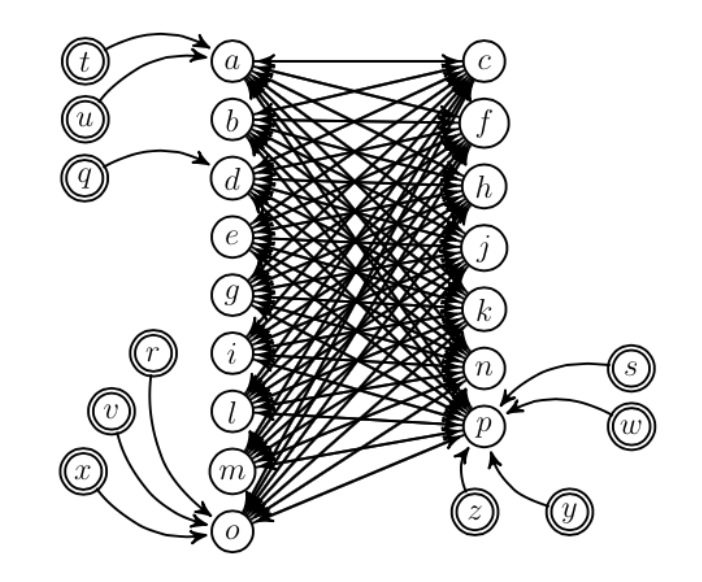
\includegraphics[width=0.5\textwidth]{argumentationframework}
\end{figure}

Dung modelled this interaction mathematically as a directed graph; with nodes representing the arguments and edges representing the attack relations between the arguments. This model of arguments and attack relations is known as an argumentation framework.

Within an argumentation framework an argument A can become inadmissible if it is attacked by another argument B. However, if B is attacked by C and becomes in admissible then A may be reinstated.

\begin{figure}[h]
\centering
\begin{tikzpicture}

\tikzset{vertex/.style = {shape=circle,draw,minimum size=1.5em}}
\tikzset{edge/.style = {->,> = latex'}}
% vertices

\node[vertex] (a) at  (0,0) {$a$};
\node[vertex] (b) at  (1.5,0) {$b$};
\node[vertex] (c) at  (3,0) {$c$};

%edges

\draw[edge] (c)  to[bend left] (b);
\draw[edge] (b)  to[bend right] (a);

\end{tikzpicture}
\caption{A is reinstated since C attacks B}
\end{figure}


\subsection{Semantics}

\subsection{Admissible Defense Sets}

\cite{vreeswijk2006algorithm}

\subsection{Knowledge Elicitation}

In order to develop expert systems a knowledge engineer must gather domain expertise. This knowledge is elicited in a number of ways. Typically the knowledge engineer is not an expert in the domain and will gather the knowledge from books, journals and other sources. It may be more efficient for the knowledge engineer to elicit a knowledge base directly from an expert by interviewing them. Although this approach is preferable it is not always possible as the expert is busy with other work and unavailable for the long periods of time required to build a knowledge base.



\subsection{Argumentation Theory Implementations}

\cite{modgil2014aspic+} presented a tutorial introduction to ASPIC+; a framework for structured argumentation that is meant to generate abstract argumentation frameworks similar to those described by Dung. Within their framework arguments could be attacked in three ways: their uncertain premises, their defeasible inferences or on the conclusions of their defeasible inferences. The authors claim that Dungs calculus is indispensable, it provides little guidance for the modelling of such a system. ASPIC+ is proposed as a framework to guide the implementation of such a system, but is not itself implemented.

Computers can be used to model arguments using visualisation techniques. An example of this is argument diagramming tools; effective aids in helping people reason about arguments. Araucaria is one such tool is described by Reed and Rowe (2001). Araucaria was designed to make argument diagramming for undergraduates easier and also to support research activities. Reed and Rowe also developed AML (Argument Markup Language) an XML based syntax for describing the structure of arguments. Unlike Dung’s argumentation framework, Araucaria represents arguments in a tree structure and the branches of this tree represent support relations as opposed to defeat relations.

Implementations of argumentation systems are more commonly based around decision support systems. A review of defeasible reasoning implementations by Bryant and Krause (2004) highlight the need for well designed empirical evaluations of implementations and formal complexity analysis to justify the practical applicability of a reasoning engine. The paper also highlights the proprietary nature of successful argumentation theory based applications preventing researchers from peer reviewing the software.

Karacapilidis and Papadias (2001) describe HERMES, a system for computer supported argumentation and decision making. HERMES also provides users with access to information from external databases to further justify their arguments. Arguments are represented using a labelling approach as opposed to a graph approach. Constraints are inserted into a discussion graph and when new constraints are introduced they are checked against existing ones.

The fact that decision support systems allow users to aggregate evidence and make decisions based on that evidence lends makes them an obvious fit for medical practitioners. Hunter and Williams (2010) developed a framework for generating inference rules to argue for and against the benefits of medical treatments based on evidence. Their work highlights the benefits of argumentation systems in abstracting away the complicated nature of medical evidence into a form more manageable for practitioners.

Longo and Hederman (2013) similarly investigated the role of argumentation theory in the implementation of decision support systems. Their work provides a comparison with machine learning. The authors developed an argumentation framework (similar to to those described by Dung) to model the breast cancer recurrence problem. The results of their experiment showed that argumentation based systems could perform as well and in some cases better than machine learning algorithms.


\section{Argument Maps Improve Critical Thinking}



%----------------------------------------------------------------------------------------
%	EVALUATION
%----------------------------------------------------------------------------------------
\section{Evaluation}

As the overall aim of the research project is to compare an implementation of defeasible reasoning with machine learning, a framework for comparing the two must be developed. This is no easy task as the techniques vary considerably in the output they will produce. For supervised machine learning the output of the experiment will be a number or a classification. These numbers and classes will already be present in the training and test data sets. For defeasible reasoning this is not the case. The implementation outputs a value that is a representation of a construct. In the experiments performed for this project, that construct is mental workload. There are many ways to measure mental workload but there is no one definitive value that can be used for comparison with this value. There is no value already present in the dataset that we can compare the output of the defeasible reasoning system with.

The following section gives an overview of the various methods used to evaluate the techniques in work by previous authors.

\subsection{Evaluation of Machine Learning Techniques}\cite{witten2005data}

There are a number of methods typically used for evaluation of machine learning techniques. Numeric predictions are evaluated similarly to many scientific experiments using statistical values such as correlation and mean absolute error. Machine learning techniques for solving classification problems are often more detailed as the costs of false positives and false negatives may be different depending on the problem. Take for example the prediction of cancer recurrence. A false positive (that it is predicted cancer will recur when it will not) will result in a patient being examined by a doctor; on the other hand a false negative would result in the missed opportunity of early diagnosis, potentially costing a life.

Machine learning techniques are typically evaluated first developing a model using a labeled `training set' of data. Once the model has been developed it can be run on a labeled `test set' of data. The performance of the technique can then be measured by comparing the values predicted by the model with the labels in the test set. The exception to this is with unsupervised machine learning as the data is unlabeled. As the purpose of unsupervised machine learning is to come up with a kind of `theory' about the data, good techniques ``make everything as simple as possible, but not simpler''. This idea is the foundation of the Minimum Discription Length Principle.

Typically the amount of data used for training and testing is limited and so techniques such as cross validation and percentage of split may be used to test and validate the model. In percentage of split the data set is divided into two groups, one for training and one for testing. Typically a higher percentage is used for training the data than testing it. In cross validation a data set is divided into groups. One group is used at a time for testing the model while the rest of the data in the set is used for training it. This technique is often referred to as N-fold cross validation where N is the number of groups the data is divided into. 

The following is a brief description of a number of measures used when evaluating the results of machine learning techniques.

\subsection{Numeric Prediction Problems}

\cite{witten2005data} explain that for practical situations the best numeric prediction method tends to perform well across all performance measures. Most performance measures tend to give an overall value for the difference between the predicted and actual value in a test set. Examples of such measure include mean-squared error, root mean-squared error and mean absolute error. As mean squared error squares the difference from the mean it tends to punish large errors more than the other measures.

Mean-squared error can be defined:

$$\frac{\sum \limits_{i=1}^n (p_{i} - a_{i})^2}{n}$$

Where $p$ are the predicted values and $a$ are the actual values.

Another performance measure used for numeric prediction problems is Pearson's Correlation Coefficient. This measures the linear correlation between the predicted value and the actual value. It differs from the other measure in that it ignores the differences in the scale of the two values.

$$\frac{S_{PA}}{\sqrt{S_{P}S_{A}}}$$

where:

$$S_{PA} = \frac{\sum _{i}(p_i - \bar{p})(a_i - \bar{a})}{n - 1}$$

$$S_{P} = \frac{\sum _{i}(p_i - \bar{p})^2}{n - 1}$$
$$S_{A} = \frac{\sum _{i}(a_i - \bar{a})^2}{n - 1}$$


\subsection{Classification Problems}

\subsection{Unsupervised ML - Minimum Description Length}

\cite{grunwald2005tutorial} gives an overview of how the Minimum Description Length Principal is used to solve the problem of model selection. Overfitting is a problem that occurs frequently with unsupervised ML techniques. Overfitting occurs when a learning technique puts too much emphasis on fitting the data exactly. As a result data points like outliers can skew the model and result in it classifying future instances of the data wrongly. A model that overfits the data will classify the dataset used to train it with very little error, however, when used on a test set will perform poorly. A simpler model may not classify the training data perfectly but will perform better on test data.

As observed earlier, a simpler theory is one that allows data to be encoded using fewer bits. This idea is born from information theory. For example, the SVG file type encodes a red circle as \lstinline{<circle cx="50" cy="50" r="40" stroke="black" stroke-width="3" fill="red" />}. This is far simpler than sending every single bit used to describe circle in raw data. From the perspective of programming MDL can be compared to Kolmogorov Complexity; the simplest theory is the one that produces the shortest computer program that will print the data.

MDL views learning as data compression; \cite{grunwald2005tutorial} defines this formally: ``for a given set of hypotheses H and data set D, we should try to find the hypothesis or combination of hypotheses in H that compresses D most.'' The best point hypothesis H to explain the data D is the one which minimizes the sum L(H) + L(D|H), where
\begin{itemize}
  \item L(H) is the length, in bits, of the description of the hypothesis; and
  \item L(D|H) is the length, in bits, of the description of the data when encoded
\end{itemize}
with the help of the hypothesis.

With this in mind it can the simple representation of constructs should be considered favourable to one that is complex.

\subsection{Evaluation of Defeasible Reasoning Implementations}

The HERMES system\cite{karacapilidis2001computer} is an implementation of Argumentation Theory that allows users to collaboratively develop arguments online and support those arguments with data. The authors evaluated their system focusing on usability. A wide variety of users such as students, researchers and medical doctors were surveyed. The participants attempted to solve two problems collaboratively using the tool and then answered questions. These questions were both about the users overall opinion of the system (ease of use, enjoyable, intention to use again) and about effectiveness of the system (task clarity, easy to read, sufficiently informative). The tool focuses on collaborative decision making and not on automated output so there is no evaluation of task performance.

Matt et al.\cite{matt2010combining} combined statistical methods with argumentation theory in order to compute trust.
%how did they do this and evaluate it?

%Discuss evaluation by longo and hederman
Generally when argumentation approaches are evaluated researchers compare the ability of the implementation to predict a value already present in the dataset. 

%----------------------------------------------------------------------------------------
%	CONCLUSIONS
%----------------------------------------------------------------------------------------

\section{Conclusions}

\chapter{Design} % Main chapter title

\label{Chapter3} % Change X to a consecutive number; for referencing this chapter elsewhere, use \ref{ChapterX}

\lhead{Chapter 3. \emph{Design}} % Change X to a consecutive number; this is for the header on each page - perhaps a shortened title

%----------------------------------------------------------------------------------------
%	SECTION 1
%----------------------------------------------------------------------------------------

In order to answer the research question posed in Chapter 1, an experiment was designed. The research question is restated here:

``To what extent can an implementation of Defeasible Reasoning enhance the representation of a construct and support prediction capacity in comparison with Machine Learning?''

In order to answer this question a number of hypotheses to be tested were defined as follows:

\begin{itemize}
  \item The defeasible measure of a construct created by an expert is better at predicting objective performance values than machine learning approaches.
  \item The construct measure of an expert will have a high concurrent validity with objective measures related to the construct.
  \item The construct measure of an expert will have a high convergent validity with existing measures for the construct.
\end{itemize}

\begin{figure}[!h]
\centering
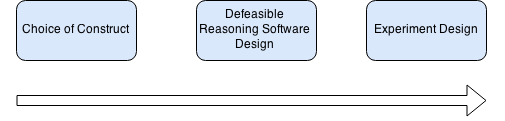
\includegraphics[width=\linewidth]{Chapter3}
\caption{Chapter Overview}
\label{fig:chapter_overview}
\end{figure}

In order to test these hypotheses the following experiments are conducted.

\begin{itemize}

  \item An argumentation system is developed in software and used to elicit a knowledge base from an expert.
  \item A number of ML classifiers (using both classification and regression algorithms) are trained to using a partition of the experiment data set.
  \item The predictive ability of the classifiers and the knowledge based system are tested using a subset of the data set.

\end{itemize}

The rest of this chapter deals with the design associated with these experiments. The choice of construct to be examined is justified, the design of the software is outlined and the experiment procedure is defined.

\section{Choice of Construct}
\label{sec:choicofc}

In order to perform the experiment a subject must be chosen. Access to an expert in the field of this subject needs to be secured as well as a data set that can be used to evaluate the representation of the construct. Suitable constructs don't have a conclusive easy to assess for of measurement such as  cancer, intelligence or personality. 

For this experiment Human Mental Workload was chosen as the construct. Mental Workload can loosely defined as the amount of effort it takes a user to perform a task. Researchers across a wide variety of domains study MWL, particularly those with interests in human performance and machine usability. \cite{meshkati2011human} outlines the problems that are associated with defining, quantifying and measuring MWL. Generalising MWL is difficult as it is a multifaceted phenomenon that varies depending on context. \cite{meshkati2011human} defines MWL as ``the operator's evaluation of the attentional load margin (between their motivated capacity and the current task demands) while achieving task performance in a mission-relevant context.'' Possible ways of measuring MWL include objectively (using task time, physiological indicators or task success) or subjectively (by having the participant answer introspective questions about their perceived state while completing the task).

One possible way of measuring MWL is using the NASA-Task Load Index (TLX). NASA-TLX is an introspective questionnaire in which participants subjectively assess their mental demand, physical demand, temporal demand, performance, effort and frustration after completing the task. Participants are then asked to compare the importance of these factors in their completion of the task. 

Another possible way to determine that MWL was high for a given task is based on the task completion time. If all variables are equal then task time can help us determine which tasks were most difficult.

Dr. Luca Longo from the DIT School of Computing is an expert in the area of MWL having completed his doctoral dissertation in formulating MWL as a defeasible construct. He has kindly volunteered his knowledge base to be used within the experiment.

The data set was obtained in an experiment performed by Dr. Longo that aimed to gather MWL information from participants based on their used of different web based interfaces. The participants had to complete 11 web based tasks using popular web applications including Google Search, Youtube and Wikipedia. 40 participants between ages 20 and 35 were split into two groups. In a given task, one group used the original application interface while the other group received a version in which the presentation of the page had been altered. Which group received the original or modified interface varied by task. It was believe that the changes to the structure of the interface would impose a greater mental workload on the participants. After each task was completed the participants answered a questionnaire designed to assess their subjective mental workload. The data set contains the results of the experiment. Sample rows are available in the appendix along with the details of each column.(\citep{longo2014formalising})

\section{Machine Learning Software}

In order to implement the experiment a suite of machine learning software needed to be procured. Designing and implementing a suite of ML algorithms is a time consuming process. Moreover, a naive implementation of ML software will result in software that performs poorly. For these reasons, it was decided to use an existing ML tool set. Proprietary options include Oracle Data Miner or SAS Enterprise Miner while open source alternatives include the R programming languge or Rapid Miner. It was decided that WEKA would be a good fit for the project. 

WEKA (Waikato Environment for Knowledge Analysis) is an open source ML workbench developed at the University of Waiko. WEKA is widely used in both academia and business. It has a simple user interface which provides feedback related to model performance in a clear and concise format. It contains implementations of machine learning algorithms across a range of typologies which allows for a large comparison with defeasible reasoning. As it is an open-source project it is possible to investigate the source code to gain a greater understanding of the underlying techniques. WEKA has a low barrier to entry; this is important to save time as a significant portion of the project will involve the implementation of defeasible reasoning software.

%----------------------------------------------------------------------------------------
%	SOFTWARE DESIGN
%----------------------------------------------------------------------------------------

\section{Defeasible Reasoning Software Design}

In order to demonstrate how DR can model a complex construct, software was designed that would allow an expert to input their knowledge base as directed graph. There is no standard way to implement a system based on defeasible reasoning. Section ~\ref{sec:dr_implementations} outlines approaches taken by others in the past to implement such systems. By drawing on these designs and identifying use cases for this project a new DR implementation can be designed. 

\subsection{Use cases}

The users of the system are both the experiment administrator and the expert/knowledge engineer. In the context of the experiment the role of knowledge engineer is played by the experimenter.

\begin{itemize}
  \item ``As an expert/KE I want to input my/a knowledge base as a defeasible construct.''
  \item ``As an expert/KE I want to model my/an expert's knowledge base in a way that will produce a numerical output given some numerical input.''
  \item ``As a system user I want to be able to save my work and retrieve work I have done previously.''
  \item ``As a system user, when I open the program what I was last working on should be displayed or a new project should open.''
  \item ``As a system user I should be able to retrieve data to test my knowledge base with. I should be able to investigate that data and investigate the results of running my knowledge-base on that data.''
  \item ``As an experimenter I should be able to collect results from running an experts knowledge-base on a full set of data.''
\end{itemize}

By investigating each of these user stories a system can be designed suitable for the purposes of the experiment.

\subsection{Defeasible Knowledge Base}
\label{sec:def_kb}
The expert or knowledge engineer must be able to model their knowledge base as a defeasible process. This process is being modeled as an Argumentation Framework as proposed by \cite{dung1995acceptability}. To reiterate, an argumentation framework is a set of arguments and attack relations between those arguments. In the case of MWL, an example of an argument is ``if the user's effort is low, this implies that the user's mental workload is low''. Another is ``if the user's performance is low, this implies that the user's mental workload is high''. It can be said that the former attacks the later since if the user doesn't make any effort the performance will be low. In the argumentation framework $S = \langle A , R \rangle A$ is the set of arguments $A = \{ a , b , c , d \}$ and R is the set of attacks $R = \{ (\, a , b )\, , (\, b , c )\, , (\, c , d )\, \}$  These arguments and attacks relations must be input into the system in a format that allows them to be processed and that allows the user to easily modify and reason about what they have input.

One method that could be adopted in designing the interface is a text based approach. The user enters their knowledge base in a text editor as a list of nodes and attack relations according to a format specified by the system designer that can be parsed by the software. An example of a JSON based format would be the following:

\begin{lstlisting}
"knowledge_base" {
    "arguments": [
                    "Low Effort->Low MWL", 
                    "High Effort->High MWL", 
                    "Low Performance->High MWL", 
                    "High Performance->Low MWL"
                ],
    "attacks":  [
        ["Low Effort->Low MWL", "Low Performance->High MWL"]
    ]
}
\end{lstlisting}

Using this approach it is easy to implement logic to parse the AF. This lightweight approach is preferable for designing test cases for the system as it is trivial for a technical user to modify and copy. 

This approach is unsustainable for regular users and large (real) knowledge bases. It is time consuming and cumbersome for a user to have to type out an argument every time that they want to create an attack. It is also intimidating for non-technical users and error-prone. As they are stored separately it can be difficult for the user to keep track of the nodes and attacks. The user would need to establish a strong naming convention to ensure that the correct arguments are attacking each other. If the user needs to store more information about the arguments and their relationships the resulting file format will grow increasingly complex.

For this reason the software has been designed to utilise a Graphical User Interface that allows a user to draw a directed graph. A user creates a new argument by clicking on an empty space on the graph. The user can name this node in order to keep track of what it represents. Once nodes have been created the user can then model the attack relations between the arguments by dragging from one node to another.

This approach has many advantages in comparison with the first approach. A non technical user will be more comfortable using a GUI than using the text based approach. When the knowledge base is input using text the user must take special care to ensure that the attack relations are correct.

There are additional requirements that need to be satisfied by the software in order to correctly model an AF. The first is the concept of rebutting attacks. In order to model rebutting attacks the user must be able to draw edges in the graph with arrows on both ends. The second is modeling the concept of mitigating arguments. Some arguments weigh in on the final evaluation of the semantic without actually contributing to the value of the construct. These arguments must be taken into consideration but have their output ignored in the final value. 

\begin{figure}[h]
    \centering
    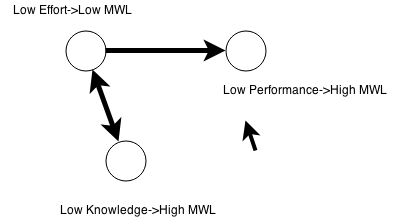
\includegraphics[width=1\textwidth]{mockup1}
    \caption{A Mockup of the UI for entering an Argumentation Framework}
    \label{fig:mesh1}
\end{figure}

\subsection{Membership Functions}

As the system is currently defined it will provide an expert with the ability to visualise their knowledge base in the form of a directed graph. The only information that can be obtained about an argument is its relationship with other arguments and its label (a natural language statement that allows the user to identify the argument and that may in some way describe the nature of the argument). 

In order that the argumentation framework can be used to compute results a number of other concepts need to be designed into the system. The notion of whether or not an argument is activated or not needs to be modeled. Argument activation allows us to consider which attack relations to take into consideration and which to discard for a particular tuple in the data set. Arguments are based on one or more premises and each premise corresponds to one column in the data set. An argument is activated if it all of its premises are relevant to a particular instance in the data. 

\begin{exmp}
If an instance had a value of 0 for effort then an argument with the premise ``Low Effort'' would be activated and an argument with the premise ``High Effort'' would be discarded. For a value of 0 effort and 0 motivation an argument with two premises ``Low Effort and Low Motivation'' would be activated. Given this same input, the argument ``High Effort and Low Motivation'' would be discarded as only one of its premises are satisfied.
\end{exmp}

The process of activating and discarding arguments results in a sub-graph of arguments relevant to the row in the database. In order to further reduce the sub-graph argumentation semantics are run on it which take into account the attack relations between the arguments. This results in a set of possible sub-graphs that are applicable to that instance in the data-set.

From the remaining arguments in each sub-graph a value for the construct being measured must be determined. These values can then be averaged for a particular graph to give an overall value for the construct for that instance. 

\begin{exmp}
If the argument is ``low performance -> high MWL'' then for a simple mapping a performance value of 0 will result in a MWL value of 100. This can be repeated for every argument and averaged for a value of MWL.
\end{exmp}

In order to determine whether or not an argument is activated we will use fuzzy sets in a manner similar to Longo and Hederman. Fuzzy Sets were defined by \cite{zadeh1965fuzzy} as ``a class of objects with a continuum of grades of membership.'' These sets are characterised by membership functions; functions that take a value and map it to a number between 0 and 1 (where 0 indicates absence of the value in the set and 1 indicates its presence.) This allows us to take a vague statement such as ``High Performance'' and determine to what extent a value of performance is considered to be high. 

For the purposes of the experiment we consider a premise to be relevant if the input value falls between the bounds of its membership function. If all associated values satisfy the membership functions of an argument, even with a very small degree of truth, then that argument is taken into consideration when evaluating the semantics of the AF for that row. If even one value associated with an arguments premise falls outside the membership function then the argument is disregarded.

By taking a value from a column the degree of truth of the premise as applied to the row can be determined using a membership function. We can then determine the overall degree of truth for an argument by computing the average of the degrees of truth of the premises. The degree of truth for the argument is then used as the input for an argument output function which determines value associated with the construct for that argument.

The following is an example of this process. Taking the argument labeled ``Low Effort \& Low Performance $\rightarrow$ Low MWL''; two premises can be identified: ``Low Effort'' and ``Low Performance'' and an output function ``Low MWL''. The premises and output function could be modeled as in figure~\ref{fig:membership_functions}. Table~\ref{tab:memfunc_ex} shows example input and output for the function. 


\begin{figure}
    \centering
        \subfigure[Low effort membership function]{\label{fig:a}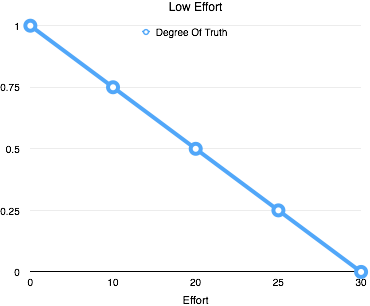
\includegraphics[width=47mm]{loweffort}}
        \subfigure[Low performance membership function]{\label{fig:b}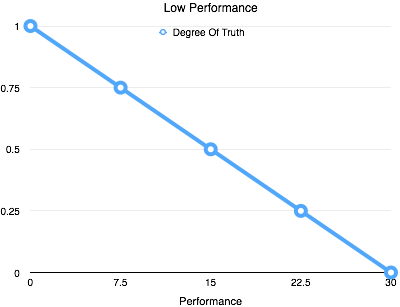
\includegraphics[width=47mm]{performance}}
         \subfigure[Output function]{\label{fig:b}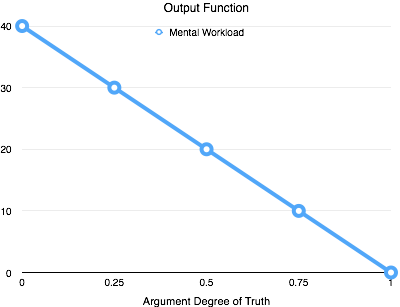
\includegraphics[width=47mm]{outputfunction}}
    \hfill
    \caption{Example membership functions and output function}
    \label{fig:membership_functions}
\end{figure}

\begin{table}[]
\begin{center}
  \begin{tabular}{ | l | l | p{8cm} |}
    \hline 
Effort & Performance & Result \\ \hline
0 & 0 & The argument's degree of truth is 1 overall, the value for MWL is 0. \\
30 & 30 & The argument's degree of truth is 0 overall, its output is considered since the input's are in range. its value for MWL is 40. \\
50 & 15 & The argument is discarded as the value for Effort is out of the range of the membership functions. \\
20 & 15 & The argument's degree of truth is .5 overall, the value for MWL is 20. \\
    \hline
  \end{tabular}
\end{center}
\caption{Caption}
\label{tab:memfunc_ex}
\end{table}

It is possible that membership functions could be input by the user in the form of mathematical functions. This would require the user has sufficient mathematical proficiency that they can express their beliefs in as mathematical functions. A more user friendly method of eliciting membership and output functions from the user is to have them draw the functions by hand using the software. We can then use the data associated with this drawing to determine the appropriate output for a given premise given a tuple in the data set.

\subsection{Additional Software Requirements}

Additional requirements specified in the user stories involve being able to retrieve and save the knowledge bases they have been working on. This is to be implemented by serealizing and deserealizing the AF into a JSON file similar in format to that described in section ~\ref{sec:def_kb}. This serialization will also be used to retrieve whatever the user was last working on when they utilise the system.

In order that a user can test their knowledge base the user will be given access to a data set. This will be displayed as a table with the user able to compute results for individual rows.

The complete design for the regular user stories has been achieved. A mock up of the resulting UI is given in figure ~\ref{fig:fullMU}.

\begin{figure}[h]
    \centering
    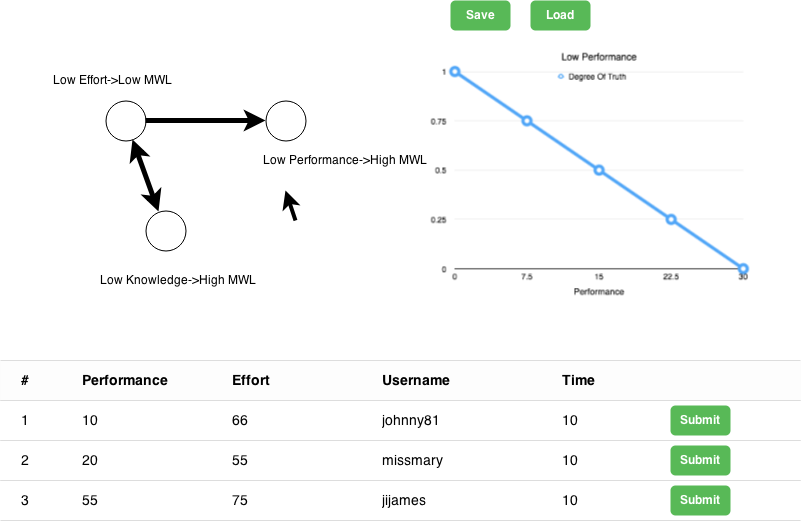
\includegraphics[width=1\textwidth]{Mockup}
    \caption{A Mockup of the UI for entering an Argumentation Framework}
    \label{fig:fullMU}
\end{figure}

In order that the experiment administrator can compute results for may knowledge bases and collect additional information, the business logic for the application is encapsulated in a class, \lstinline{FrameworkRunner}. This allows it to be called from both the GUI and a command line interface with additional options.

\section{Experiment Procedure}

Now that the necessary software for the experiment has been designed a formal procedure for undertaking the experiment can be defined. The research question referred to at the beginning of this chapter needs to be reinterpreted in the context of mental workload. With respect to predictive capacity an attempt will be made to answer the following question: ``Given data associated with an individual undertaking a task can we predict their mental workload?'' 

We will attempt to answer this question by performing four sub-experiments. Each experiment will examine a different technique's ability to model and predict MWL based on the data set that has been provided. An experiment will be performed for Supervised ML continuous techniques, Supervised ML discrete techniques, Unsupervised ML and Defeasible Reasoning. All of the techniques will be required to make their inferences based on the following data set columns: mental, temporal, psychological, performance, effort, central, response, visual, auditory, spatial, verbal, manual, speech, arousal, bias, intention, knowledge, parallelism, skill, difficulty. 

What is important to note, as explained in section ~\ref{sec:choicofc} is that there is no concrete definition of what MWL is. Each technique will have a different interpretation of what MWL really ``means''. As a result there is no yardstick we can objectively measure the results against and say that one technique is inconclusively better than the other. The results will be evaluated both quantitatively and qualitatively in the context of the material gathered in the literature review.

In order to test ML techniques for predicting numerical outputs, some measure of a construct must already be present in the data used for training and testing. For this reason MWL is interpreted to be equivalent to task time. Time on task is often used in usability experiments to determine the usability of a computer interface. This approach has several flaws which will be the subject of further discussion in the evaluation chapter.

Similarly for the classification techniques, the construct must be interpreted as some label in the data. There is a relationship between MWL and the task ID, some tasks were designed to produce greater MWL than others. Thus in this experiment task ID is interpreted as MWL.

The unsupervised ML techniques will produce subsets of the data. These can be compared against the results of the other experiments to yield some insight into MWL.

For each of the ML techniques mentioned a number of common algorithms of that category are chosen. Each algorithm is run on the data using Weka. The output from each iteration of the experiment are the models developed by the algorithm and statistics about the performance of the model. All of the supervised ML algorithms are trained and evaluated on the dataset using 10-fold cross validation. The results of each iteration are collected and stored for analysis later.

The last experiment to be conducted involves determining the defeasible reasoning software implementation's capacity to model and predict a construct. The software is implemented and then used by to elicit the knowledge base of both an expert and a lay person with regards to MWL. The participant evaluates their knowledge base using a portion of the data set. The results of running the knowledge base using DR techniques are then collected by the experiment implementer. Within this experiment a completely new value for MWL is developed based on the participants beliefs. The experiment also returns a degree of truth for MWL value and some performance characteristics of the software. These results may then be evaluated with respect to each other and the results from the other experiments. 

\section{Conclusions}

This chapter presented the experiment being undertaken to evaluate the hypothesis of this research project. The experiment will consist of a test of machine learning methods and defeasible reasoning techniques. In order to establish how the research question will be tested the idea of a construct was defined. The construct for the experiment was chosen to be mental workload and an experiment for determining the ability of different techniques to model this construct was designed.

A necessary step in performing this experiment is the implementation of a defeasible reasoning system. The design of this software is influenced by the implementation created by  \cite{longo2012argumentation}; however it build upon this work by offering a GUI that allows the implementation to be used for modeling multiple phenomena as defeasible processes. A software design is outlined order to undertake the defeasible reasoning portion of the evaluation. The design of the software includes the requirements for the user to be able to draw an argumentation framework that models their knowledge base and determine activation of the arguments within that framework by drawing membership functions.
% Chapter Template

\chapter{Implementation} % Main chapter title

\label{Chapter4} % Change X to a consecutive number; for referencing this chapter elsewhere, use \ref{ChapterX}

\lhead{Chapter X. \emph{Chapter Title Here}} % Change X to a consecutive number; this is for the header on each page - perhaps a shortened title

%----------------------------------------------------------------------------------------
%	SECTION 1
%----------------------------------------------------------------------------------------

\section{Introduction}

In order to perform the experiment it was necessary to implement the defeasible reasoning software as designed in the previous chapter.  
%   \begin{figure}[h!]
% \begin{center}
% \begin{tikzpicture}[->,>=stealth',shorten >=1pt,auto,node distance=2.5cm, semithick, scale=0.95, ,transform shape, align=left] 
% \tikzstyle{every state}=[fill=white,draw=black,text=black, font=\tiny, minimum size=5mm] 
%  \tikzstyle{EdgeStyle}=[bend left, font=\tiny] 
 
%  %central
% \node[state] at(-8,1) (SD1) {SD1}; 
% \node[state] at(-7,0) (SD2) {SD2};
% \node[state] at(-6,0) (SD3) {SD3};
% \node[state] at(-5,1) (SD4) {SD4};

% %mental demand
% \node[state] at(-8,2) (MD1) {MD1};
% \node[state] at(-7,3) (MD2) {MD2};
% \node[state] at(-6,3) (MD3) {MD3};
% \node[state] at(-5,2) (MD4) {MD4};

% %context bias
% \node[state] at(-8,4.5) (CB1) {CB1};
% \node[state] at(-7,4) (CB2) {CB2};
% \node[state] at(-6,4) (CB3) {CB3};
% \node[state] at(-5,4.5) (CB4) {CB4};

% %stress
% \node[state] at(-7,5.5) (PS1) {PS1};
% \node[state] at(-6,5.5) (PS2) {PS2};

% %effort
% \node[state] at(-8,8) (EF1) {EF1};
% \node[state] at(-7,8) (EF2) {EF2};
% \node[state] at(-6,8) (EF3) {EF3};
% \node[state] at(-5,8) (EF4) {EF4};

% %
% \node[state] at(-4,7) (DS1) [double] {DS1};


% %motivation mitigating
% \node[state] at(-8,6.5) (MV3) [double] {MV3};
% \node[state] at(-7,6.5) (MV5) [double] {MV5};
% \node[state] at(-5,6.5) (MV2) [double] {MV2};
% \node[state] at(-6,6.5) (MV4) [double] {MV4};


% %motivation forecast
% \node[state] at(-6,9.5) (MV1) {MV1};


% %past knowledge
% \node[state] at(-7,9.5) (PK1) {PK1};
% \node[state] at(-5.5,11.5) (PK2) {PK2};

% %skills
% \node[state] at(-8,10) (SK1) {SK1};
% \node[state] at(-7.0,11.5) (SK2) {SK2};

% \node[state] at(4,11.5) (SR1) {SR1};
% \node[state] at(3,11.5) (SR2) {SR2};
% \node[state] at(2,11.5) (SR3) {SR3};
% \node[state] at(1,11.5) (SR4) {SR4};

% \node[state] at(-1,11.5) (TS1) {TS1};
% \node[state] at(-2,11.5) (TS2) {TS2};
% \node[state] at(-3,11.5) (TS3) {TS3};
% \node[state] at(-4,11.5) (TS4) {TS4};

% \node[state] at(3.8,0) (VM1) {VM1};
% \node[state] at(2.8,0) (VM2) {VM2};
% \node[state] at(1.8,0) (VM3) {VM3};
% \node[state] at(0.8,0) (VM4) {VM4};

% \node[state] at(-1,0) (VR1) {VR1};
% \node[state] at(-2,0) (VR2) {VR2};
% \node[state] at(-3,0) (VR3) {VR3};
% \node[state] at(-4,0) (VR4) {VR4};

% \node[state] at(-3.8,2.5) (AR1) {AR1};
% \node[state] at(-2.8,2.5) (AR2) {AR2};
% \node[state] at(-1.8,2.5) (AR3) {AR3};
% \node[state] at(-0.8,2.5) (AR4) {AR4};

% \node[state] at(4,1.5) (MR1) {MR1};
% \node[state] at(3,1.5) (MR2) {MR2};
% \node[state] at(2,1.5) (MR3) {MR3};
% \node[state] at(1,1.5) (MR4) {MR4};

% %
% \node[state] at(-0.5,1.3) (SP1) {SP1};
% \node[state] at(-1.5,1.3) (SP2) {SP2};
% \node[state] at(-2.5,1.3) (SP3) {SP3};
% \node[state] at(-3.5,1.3) (SP4) {SP4};


% %
% \node[state] at(-3.5,10.5) (TD1) {TD1};
% \node[state] at(-2.5,10.5) (TD2) {TD2};
% \node[state] at(-1.5,10.5) (TD3) {TD3};
% \node[state] at(-0.5,10.5) (TD4) {TD4};

% %
% \node[state] at(-2,6) (PF1) {PF1};
% \node[state] at(-2,9.3) (PF2) {PF2};
% \node[state] at(2,10) (PF3) {PF3};
% \node[state] at(2,6) (PF4) {PF4};

% %
% \node[state] at(3.8,2.8) (PA1) {PA1};
% \node[state] at(2.8,2.8) (PA2) {PA2};
% \node[state] at(1.8,2.8) (PA3) {PA3};
% \node[state] at(0.8,2.8) (PA4) {PA4};

% \node[state] at(4,6) (AD1a) [double] {AD1a};
% \node[state] at(4,5) (AD2a) [double] {AD2a};
% \node[state] at(3.0,4) (AD6c) [double] {AD6c};
% \node[state] at(1,4) (AD5c) [double] {AD5c};
% \node[state] at(0.5,6.3) (AD3b) [double] {AD3b};
% \node[state] at(3.5,7) (AD4f) [double] {AD4f};
% \node[state] at(1.2,7.5) (AD4c) [double] {AD4c};



% \node[state] at(-4.2,5.5) (AD3a) [double] {AD3a};
% \node[state] at(-3.6,4) (AD4a) [double] {AD4a};
% \node[state] at(-1.8,4) (AD5a) [double] {AD5a};
% \node[state] at(-0.3,4) (AD5d) [double] {AD5d};
% \node[state] at(-0.1,5) (AD4d) [double] {AD4d};

% \node[state] at(-3,7) (DS2) [double] {DS2};
% \node[state] at(-1,7) (DS3) [double] {DS3};
% \node[state] at(-0.5,6) (DS4) [double] {DS4};


% \node[state] at(4,9) (AD5f) [double] {AD5f};
% \node[state] at(4,10.5) (AD4e) [double] {AD4e};
% \node[state] at(1,10.5) (AD6b) [double] {AD6b};
% \node[state] at(1,9) (AD1b) [double] {AD1b};



% \node[state] at(-3.5,8) (AD5b) [double] {AD5b};
% \node[state] at(-2,8) (AD5e) [double] {AD5e};
% \node[state] at(2.3,8) (AD2b) [double] {AD2b};
% \node[state] at(3.5,8) (AD4b) [double] {AD4b};
% \node[state] at(-4,9) (AD6a) [double] {AD6a};
% \node[state] at(-0,9) (AD1c) [double] {AD1c};
% \node[state] at(0,7.5) (AD2c) [double] {AD2c};

% %\path
% %(MV3) [bend left, ->,  dashed] edge  node {uc3} (EF1)
% %(MV5) [bend left, ->,  dashed] edge node {uc4}  (EF2)
% %(MV4) [bend left, ->,  dashed] edge node {uc1}  (EF3)
% %(MV2) [bend left, ->,  dashed] edge node {uc2} (EF4)
% %(AD3a) [bend left, ->,  dashed] edge node {um7} (PF1)
% %(AD4a) [bend left, ->,  dashed] edge node {um9} (PF1)
% %(AD5a) [bend left, ->,  dashed] edge node {um15} (PF1)
% %(AD4d) [bend left, ->,  dashed] edge node {um12} (PF1)
% %(AD5d) [bend left, ->,  dashed] edge node {um18} (PF1)
% %(AD1c) [bend left, ->,  dashed] edge node {um3} (PF2)
% %(AD2c) [bend left, ->,  dashed] edge node {um6} (PF2)
% %(AD5b) [bend left, ->,  dashed] edge node {um16} (PF2)
% %(AD5e) [bend left, ->,  dashed] edge node {um19} (PF2)
% %(AD6a) [bend left, ->,  dashed] edge node {um21} (PF2)
% %(AD1b) [bend left, ->,  dashed] edge node {um2} (PF3)
% %(AD2b) [bend left, ->,  dashed] edge node {um4} (PF3)
% %(AD4b) [bend left, ->,  dashed] edge node {um10} (PF3)
% %(AD5f) [bend left, ->,  dashed] edge node {um20} (PF3)
% %(AD6b) [bend left, ->,  dashed] edge node {um22} (PF3)
% %(AD5c) [bend left, ->,  dashed] edge node {um17} (PF4)
% %(AD4e) [bend left, ->,  dashed] edge node {um13} (PF3)
% %(AD1a) [bend left, ->,  dashed] edge node {um1} (PF4)
% %(AD2a) [bend left, ->,  dashed] edge node {um4} (PF4)
% %(AD3b) [bend left, ->,  dashed] edge node {um8} (PF4)
% %(AD4c) [bend left, ->,  dashed] edge node {um11} (PF4)
% %(AD4f) [bend left, ->,  dashed] edge node {um14} (PF4)
% %(AD6c) [bend left, ->,  dashed] edge node {um23} (PF4)
% %(DS2) [bend left, ->,  dashed] edge node {uc6} (PF1)
% %(DS3) [bend left, ->,  dashed] edge node {uc7} (PF1)
% %(DS4) [bend left, ->,  dashed] edge node {uc8} (PF1)
% %(DS1) [bend left, ->,  dashed] edge node {uc5} (EF4)
% %(MD1) [bend left, <->, solid] edge node {r1} (SD4)
% %(MD4) [bend left, <->] edge node {r2} (SD1)
% %(PK1) [bend left, <->] edge node {r3} (SK2)
% %(PK2) [bend left, <->] edge node {r4} (SK1)
% %(PK1) [bend right, <->] edge node {r5} (EF1)
% %(PK2) [bend left, <->] edge node {r6} (EF4)
% %(SK1) [bend right, <->] edge node {r7} (EF1)
% %(SK2) [bend left, <->] edge node {r8} (EF4)
% %(CB4) [bend left, <->] edge node {r9} (PS1)
% %; 

% \path
% (MV3) [bend left, ->,  dashed] edge  node {} (EF1)
% (MV5) [bend left, ->,  dashed] edge node {}  (EF2)
% (MV4) [bend left, ->,  dashed] edge node {}  (EF3)
% (MV2) [bend left, ->,  dashed] edge node {} (EF4)
% (AD3a) [bend left, ->,  dashed] edge node {} (PF1)
% (AD4a) [bend left, ->,  dashed] edge node {} (PF1)
% (AD5a) [bend left, ->,  dashed] edge node {} (PF1)
% (AD4d) [bend left, ->,  dashed] edge node {} (PF1)
% (AD5d) [bend left, ->,  dashed] edge node {} (PF1)
% (AD1c) [bend left, ->,  dashed] edge node {} (PF2)
% (AD2c) [bend left, ->,  dashed] edge node {} (PF2)
% (AD5b) [bend left, ->,  dashed] edge node {} (PF2)
% (AD5e) [bend left, ->,  dashed] edge node {} (PF2)
% (AD6a) [bend left, ->,  dashed] edge node {} (PF2)
% (AD1b) [bend left, ->,  dashed] edge node {} (PF3)
% (AD2b) [bend left, ->,  dashed] edge node {} (PF3)
% (AD4b) [bend left, ->,  dashed] edge node {} (PF3)
% (AD5f) [bend left, ->,  dashed] edge node {} (PF3)
% (AD6b) [bend left, ->,  dashed] edge node {} (PF3)
% (AD5c) [bend left, ->,  dashed] edge node {} (PF4)
% (AD4e) [bend left, ->,  dashed] edge node {} (PF3)
% (AD1a) [bend left, ->,  dashed] edge node {} (PF4)
% (AD2a) [bend left, ->,  dashed] edge node {} (PF4)
% (AD3b) [bend left, ->,  dashed] edge node {} (PF4)
% (AD4c) [bend left, ->,  dashed] edge node {} (PF4)
% (AD4f) [bend left, ->,  dashed] edge node {} (PF4)
% (AD6c) [bend left, ->,  dashed] edge node {} (PF4)
% (DS2) [bend left, ->,  dashed] edge node {} (PF1)
% (DS3) [bend left, ->,  dashed] edge node {} (PF1)
% (DS4) [bend left, ->,  dashed] edge node {} (PF1)
% (DS1) [bend left, ->,  dashed] edge node {} (EF4)
% ;

% \path
% (MD1) [bend left, <->, solid] edge node {} (SD4)
% (MD4) [bend left, <->] edge node {} (SD1)
% (PK1) [bend left, <->] edge node {} (SK2)
% (PK2) [bend left, <->] edge node {} (SK1)
% (PK1) [bend right, <->] edge node {} (EF1)
% (PK2) [bend left, <->] edge node {} (EF4)
% (SK1) [bend right, <->] edge node {} (EF1)
% (SK2) [bend left, <->] edge node {} (EF4)
% (CB4) [bend left, <->] edge node {} (PS1)
% ; 

% \end{tikzpicture} 
 
% \caption{The brand new instance: Knowledge-base translated into an argumentation graph}
% \label{fig:knowledgebaseargframework}
% \end{center}
% \end{figure}

%-----------------------------------
%	SUBSECTION 1
%-----------------------------------
\subsection{Subsection 1}



%-----------------------------------
%	SUBSECTION 2
%-----------------------------------

\subsection{Subsection 2}

%----------------------------------------------------------------------------------------
%	SOFTWARE IMPLEMENTATION
%----------------------------------------------------------------------------------------

\section{Software Implementation}

It was decided that the software would be implemented as a web application. This meant that the software could be accessed remotely from a number of different devices and would allow the expert to develop their knowledge base without having the software installed on their local machine. It also meant that the experimenter had access to the experts knowledge bases that had been saved to the system.

%-----------------------------------
%	SYSTEM ARCHITECTURE
%-----------------------------------
\subsection{System Architecture}

The implementation of the application uses a Javascript based front end with a RESTful Web Service based back-end written in PHP (using the Slim framework) and Java. 

The RESTful Web Service back-end provides a number of basic functions for the application. The back-end saves a knowledge base to disk as a JSON file and can similarly retrieve a list of knowledge bases and an individual knowledge base for the user. Knowledge bases were saved as JSON on disk rather than in a database as it eased the development process and would allow a knowledge base to be examined in it's complete form without needing assemble it with queries from the database. The back-end also allows the expert to load a small number of rows from the experiment data-set in order to evaluate the correctness of their knowledge-base.

The most important function of the back-end is to take a row from the data set and compute the value of the construct using the knowledge-base. The details of how this occurs are outlined later in this chapter.

%-----------------------------------
%	SYSTEM ARCHITECTURE
%-----------------------------------
\subsection{Application Front End}

A number of frameworks and libraries have been utilised in the development of the front-end. Bootstrap and JQuery have been used for presentational aspects of the site. Bootstrap provides a number of different useful components such as modal boxes allow the software to present information to the user in a clear manner. JQuery provides functionality such as DOM manipulation and AJAX networking facilities. 
A crucial component of the software is the development of argumentation frameworks and membership functions. This is achieved using the D3 library developed by Bostock et al.\cite{2011-d3} D3.js is a data visualisation library that allows developers and designer to load data and interact with the DOM using the data. Two key functionalities of D3 that are used in the implementation of the software are it's implementation of Bezier curves and it's force directed graph implementation.

Force directed graphs attempt to solve the problems posed when visualising graph data structures. Typical data visualisation techniques take values and parse them one by one, drawing some value in a position, drawing the next value next to it and so forth. This is not the case in graph data structures as generally it is prefered to have vertices that have common edges close together and to have those without common edges far apart. D3 provides a solution to this problem in the form of it's force directed techniques. The techniques take list of vertices and edges and generate positions for vertices using simulation inspired by physics. Similarly to sub-atomic particles, nodes are given a charge that repel other nodes in the graph. Nodes are from drifting apart by the links in the graph. There is also a force at the center of the visualisation that any of the nodes from drifting outside the viewport. 

The algorithms for generating the positions of the nodes are implemented in the D3 `force' layout. By utilising this layout and D3's event helpers (listeners for mouse actions such as click and drag) an interface can be implemented that allows a user to input a directed graph. This is the implementation that allows an expert to input an abstract argumentation framework.

By selecting a node in the graph representing an argument a user can then define membership functions representing premises and an output function. They do this by manipulating control points on a Bezier curve. D3 allows us to draw these curves and control points using SVG, which defines it's `paths' (Bezier curves) using control points. The membership functions and output function are defined simply as control points in the data model. The server uses algorithms to compute an output given an input value and a set of control points. In order to make these algorithms accessible to the reader a brief explanation of Bezier curves follows.

%-----------------------------------
%	BEZIER CURVES
%-----------------------------------

\subsection{Bezier Curves}

A Bezier Curve is a curve produced by a parameterised equation that produces a 

\subsection{Backend Implementation}

The basic functions of the backend such as storage and retrieval of data have been explained in section 1 of this chapter. The most crucial function of the back end is to take a row in the dataset and determine what a value for the construct associated with that row based on the knowledge base. In order to do this the javascript client makes a HTTP Post request to the base URL of the backend. This post request contains a JSON object which includes the expert's knowledge base, the row in the dataset and a list of semantics that are to be computed.

Once this request is parsed by the backend, irrelevant arguments and their associated links are removed from the graph. This is achieved by looking at an arguments membership functions. If the row in the dataset doesn't have a value between the minimum and maximum value of all premises in the argument then this argument is not activated and can be removed.

\begin{algorithm}
\caption{Determine activated arguments}
\begin{algorithmic} 
\FOR{each argument $arg$ \Pisymbol $N$ }
    % \FOR{each membership function $prem$ \Pisymbol{psy}{206} $arg$}
    %     $Val$ \leftarrow the column in the data corresponding to the premise
    %     \IF{$Val$ < $prem$\rightarrow$min$ OR $Val$ > $prem$\rightarrow$max$}
    %         Remove($arg$)
    %     \ENDIF
    % \ENDFOR
\ENDFOR
\end{algorithmic}
\end{algorithm}

The sub-graph of activated arguments and their relationships produced by this step is then formatted and passed into a Java program that computes the semantics. The main functionality of this code is known as the Dung-o-matic and is released under the Apache License, Version 2.0. The Dung-o-matic is an efficient implementation of a Dung argumentation framework that is used in this project to compute the semantics of the graph. The Dung-o-matic is wrapped in a main function that takes three command line arguments: an array of nodes, and array of links between nodes and a list of semantics to be computed. This program has been exported as a JAR file which is then called from PHP using the \lstinline{exec()} function. The Java code returns JSON object with the semantic names as keys and the sub-graphs as an array of arrays associated with those keys.

Once the semantics have been computed for an Argumentation Framework the values associated with each argument can be computed. For a given row in the data set, the results for an argument remain the same no mater what the configuration of the framework is. This allows us to cache the output value of an argument in memory rather than having to recompute the same values for each semantic. The results are computed on the server using a bBzier curve implementation.

If the output function of an argument is labeled as a mitigating argument then that argument is ignored.

%scaling of bezier curves

For a given membership function with fixed values for it's control points any point on the curve can be described by a value t between 0 and 1. By passing t into the function we obtain a value for x and y. As it is not possible to simply pass in an x value and obtain a corresponding y value we must search for y by varying the parameter t. This is done efficiently using a binary search algorithm. For each iteration we pass in two values of t to get two values of x and compare them with our target x value. We continue to search a space closer and smaller to x until we arrive at a value that is within a threshold we consider to be satisfactory. The value of t at this point gives the y value.

This calculation is performed for each membership function in the node and an average of the values of the output is produced. This corresponds to the overall degree of truth for the argument. This value is then used as the input to the output function which computes an overall construct value for that argument. 

Once the all of the construct values and degrees of truth are taken the averages of both values are taken. These are considered to be the Degree of Truth of that semantic and the construct value for that semantic. This is returned along with a list of the arguments for that semantic to the client. The client presents this to the user so that the user can evaluate whether or not their knowledge base is behaving in a manner that they expect it to or not.

% Semantic algorithms

%-----------------------------------
%	EXPERIMENT IMPLEMENTATION
%-----------------------------------
\section{Experiment Implementation}

The software implemented as above was used by both an expert in mental work load and a lay person. Both were asked to describe their knowledge of mental workload as a defeasible knowledge base and the knowledge bases were collected on the server.

As computing the semantics for an AF is an NP complete problem it is not yet possible to compute the results for a whole data set in the time that it would take to complete a typical HTTP request-response cycle. For the purposes of the experiment the functionality to compute the results for a whole data set using a given knowledge base was wrapped in a command line tool written in PHP. In order to reduce the time taken to compute the results and so as to focus the analysis of the experiment only the grounded and preferred extensions were computed. These overall degree of truth for the semantic and the value of MWL for the row in the dataset were stored for later analysis.

%-----------------------------------
%	SUBSECTION 1
%-----------------------------------
\subsection{Weka}



%-----------------------------------
%	SUBSECTION 2
%-----------------------------------

\subsection{Knowledge Base Elicitation}

\begin{figure}[H]
\centering
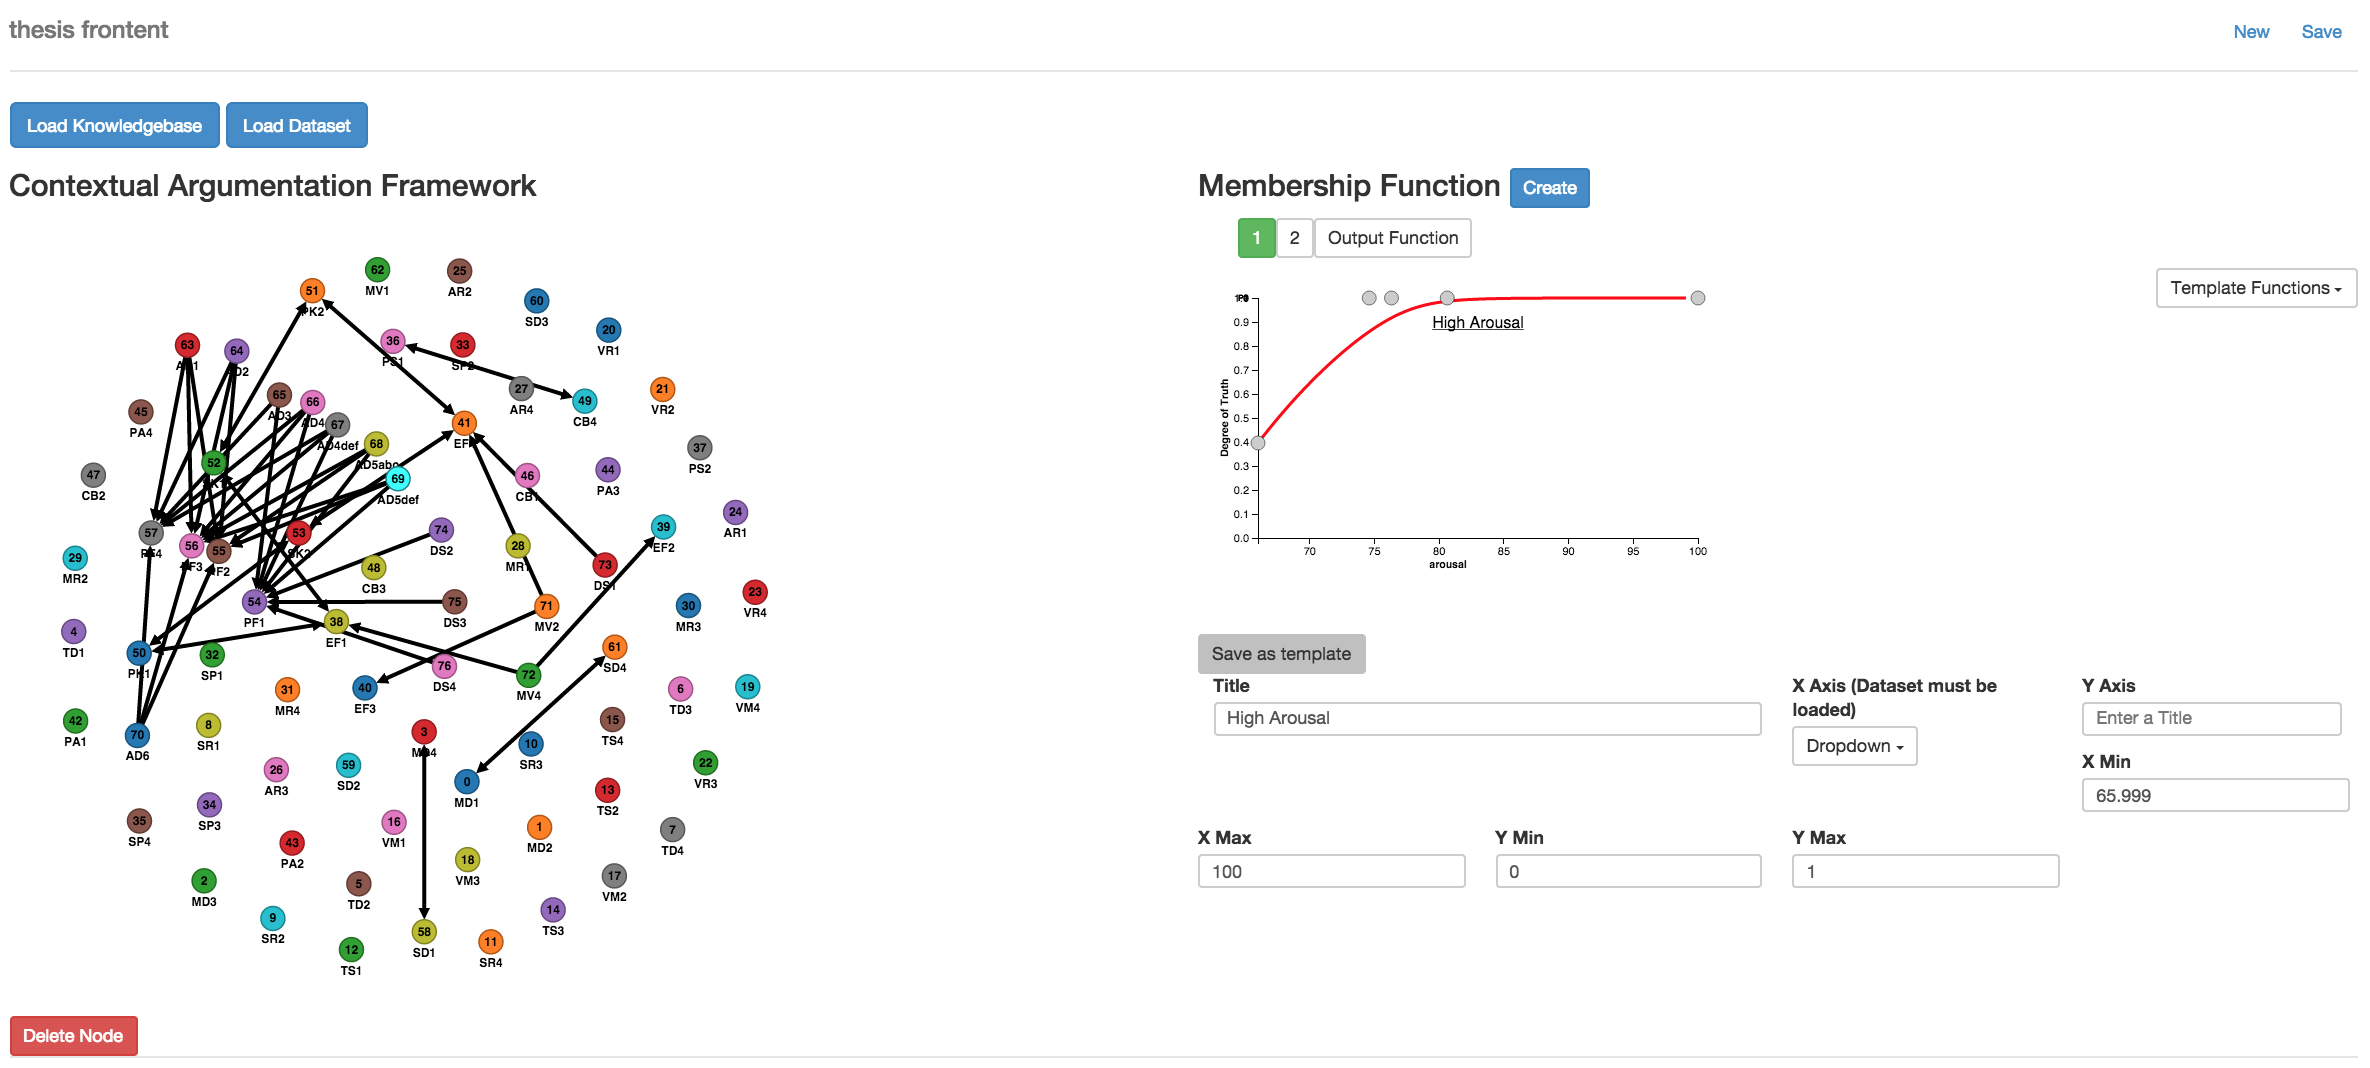
\includegraphics[width=1\textwidth]{Fullscreen}
\caption{The fully developed tool for eliciting knowledge bases}
\end{figure}

\begin{figure}[H]
\centering
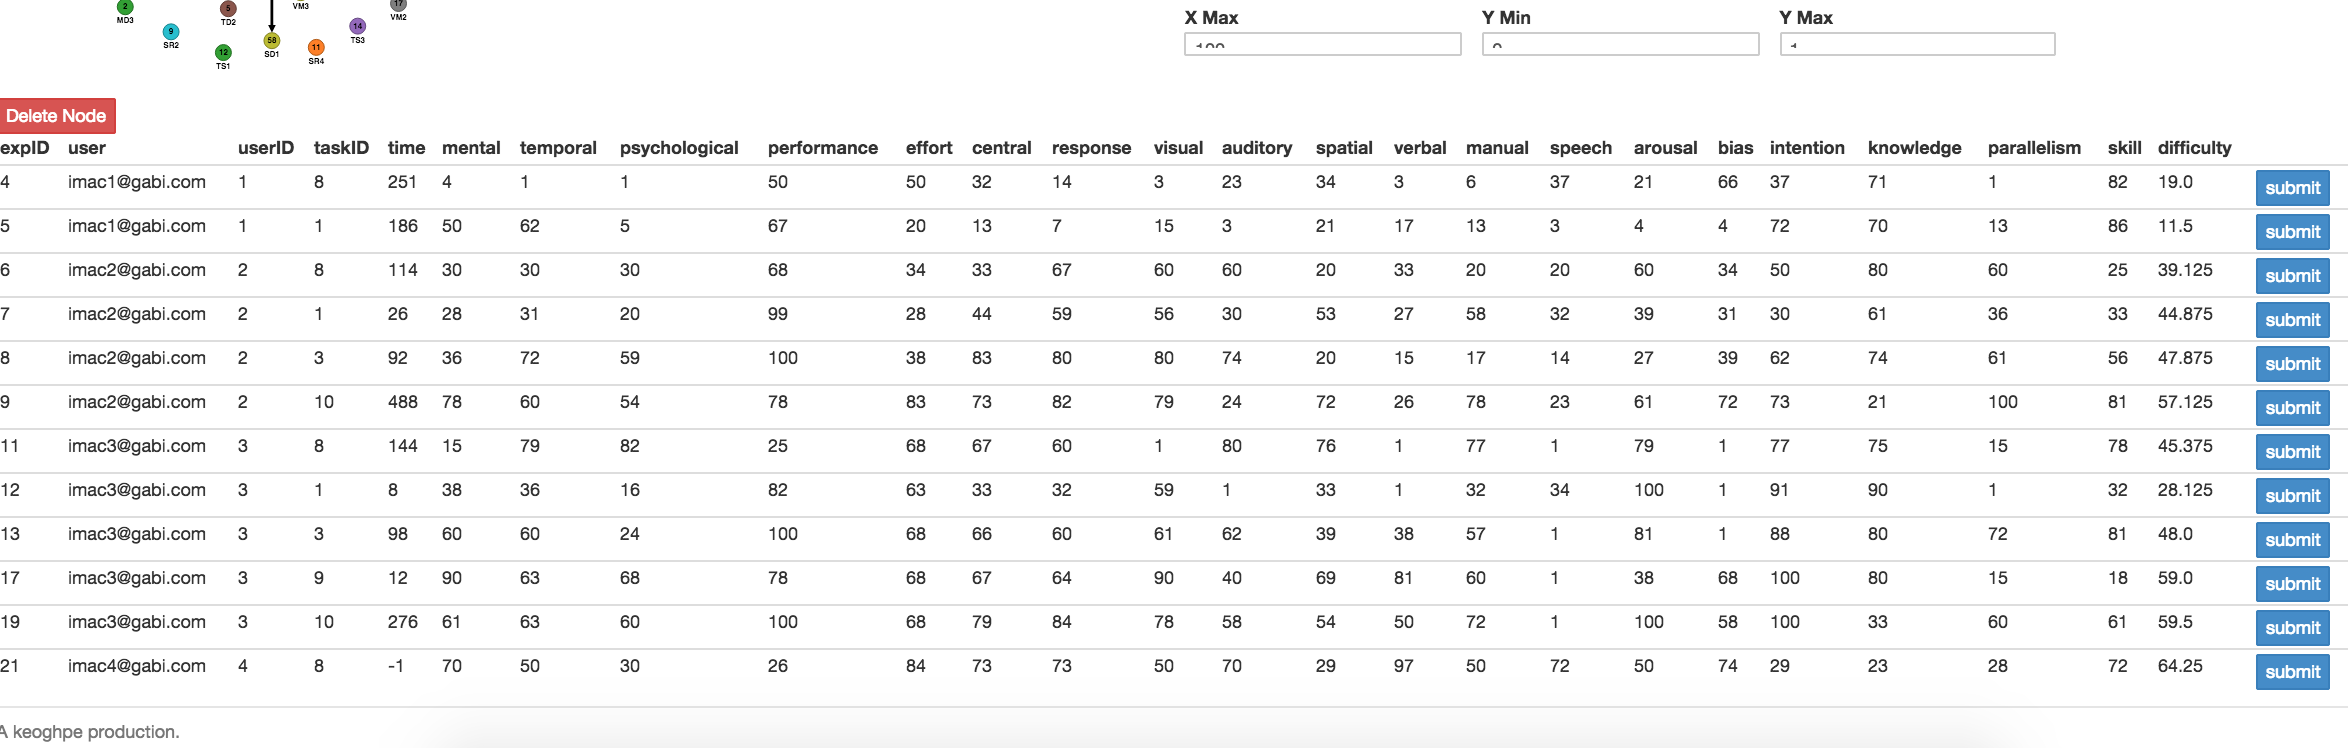
\includegraphics[width=1\textwidth]{data}
\caption{A selection of data for the user to test their knowledge base with}
\end{figure}

\begin{figure}[H]
\centering
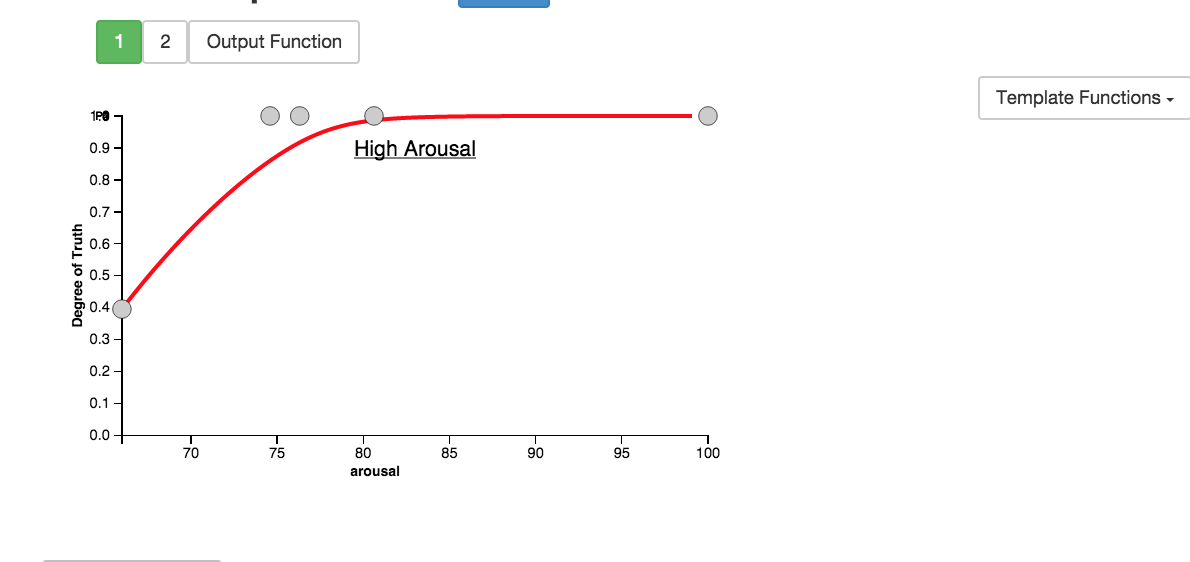
\includegraphics[width=1\textwidth]{membershipfunction}
\caption{An interface that allows a user to `draw' a membership function}
\end{figure}

\begin{figure}[H]
\centering
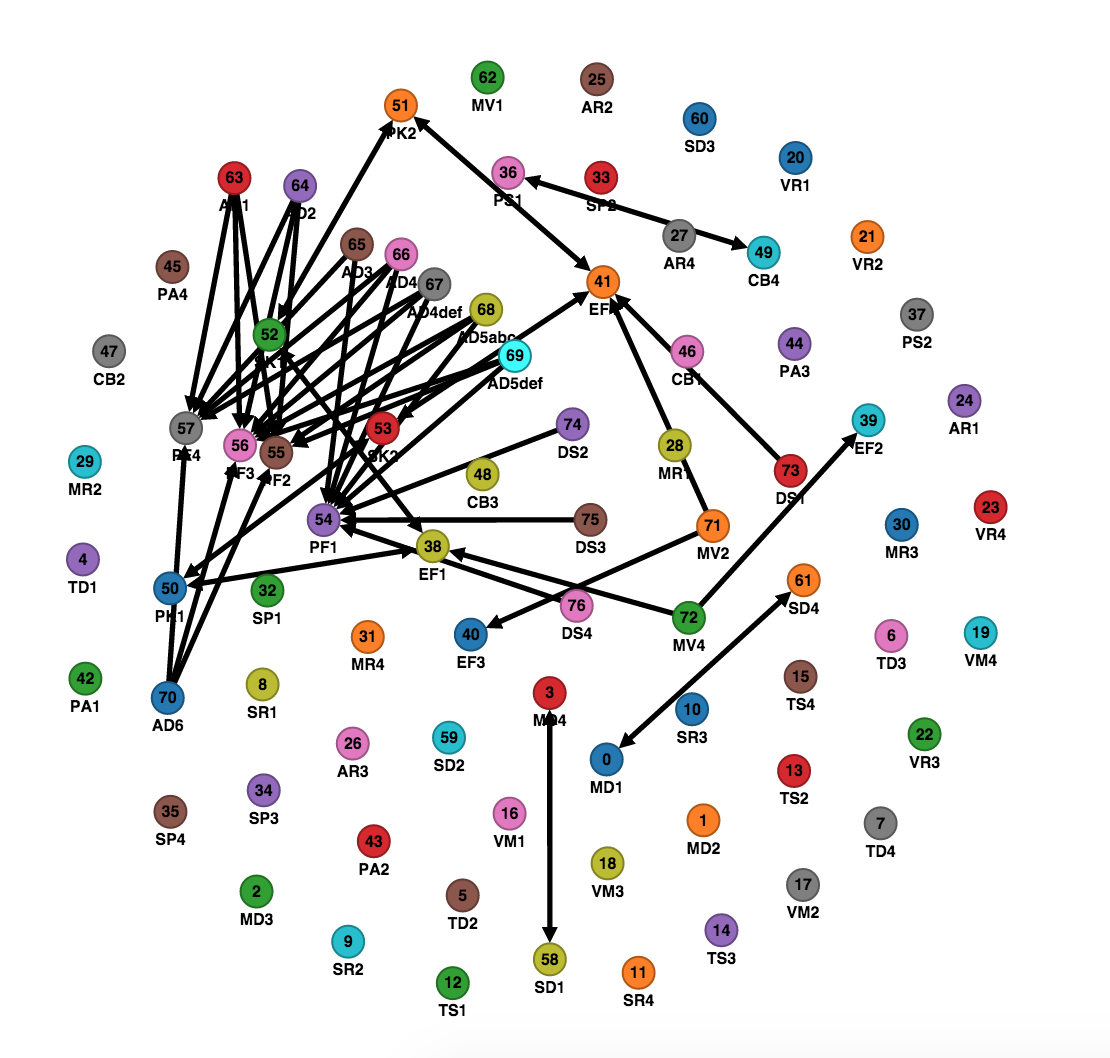
\includegraphics[width=1\textwidth]{ExpertAF}
\caption{The Argumentation Framework developed by the expert using the tool}
\end{figure}

\begin{figure}[H]
\centering
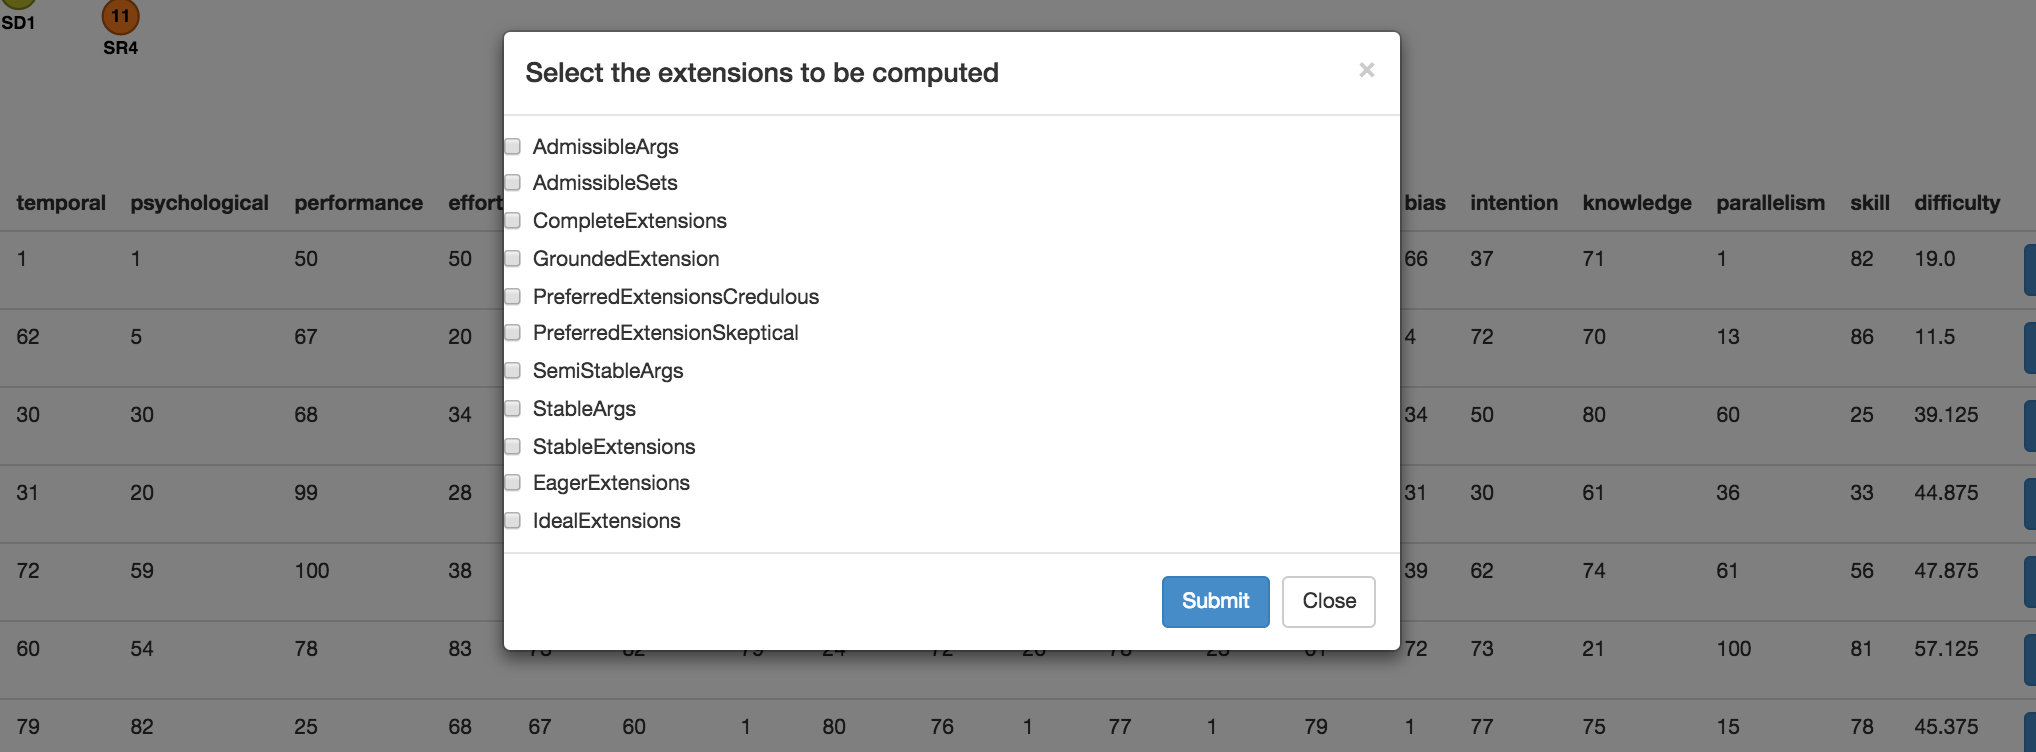
\includegraphics[width=1\textwidth]{options}
\caption{A list of options for semantics that can be computed by the system}
\end{figure}

\begin{figure}[H]
\centering
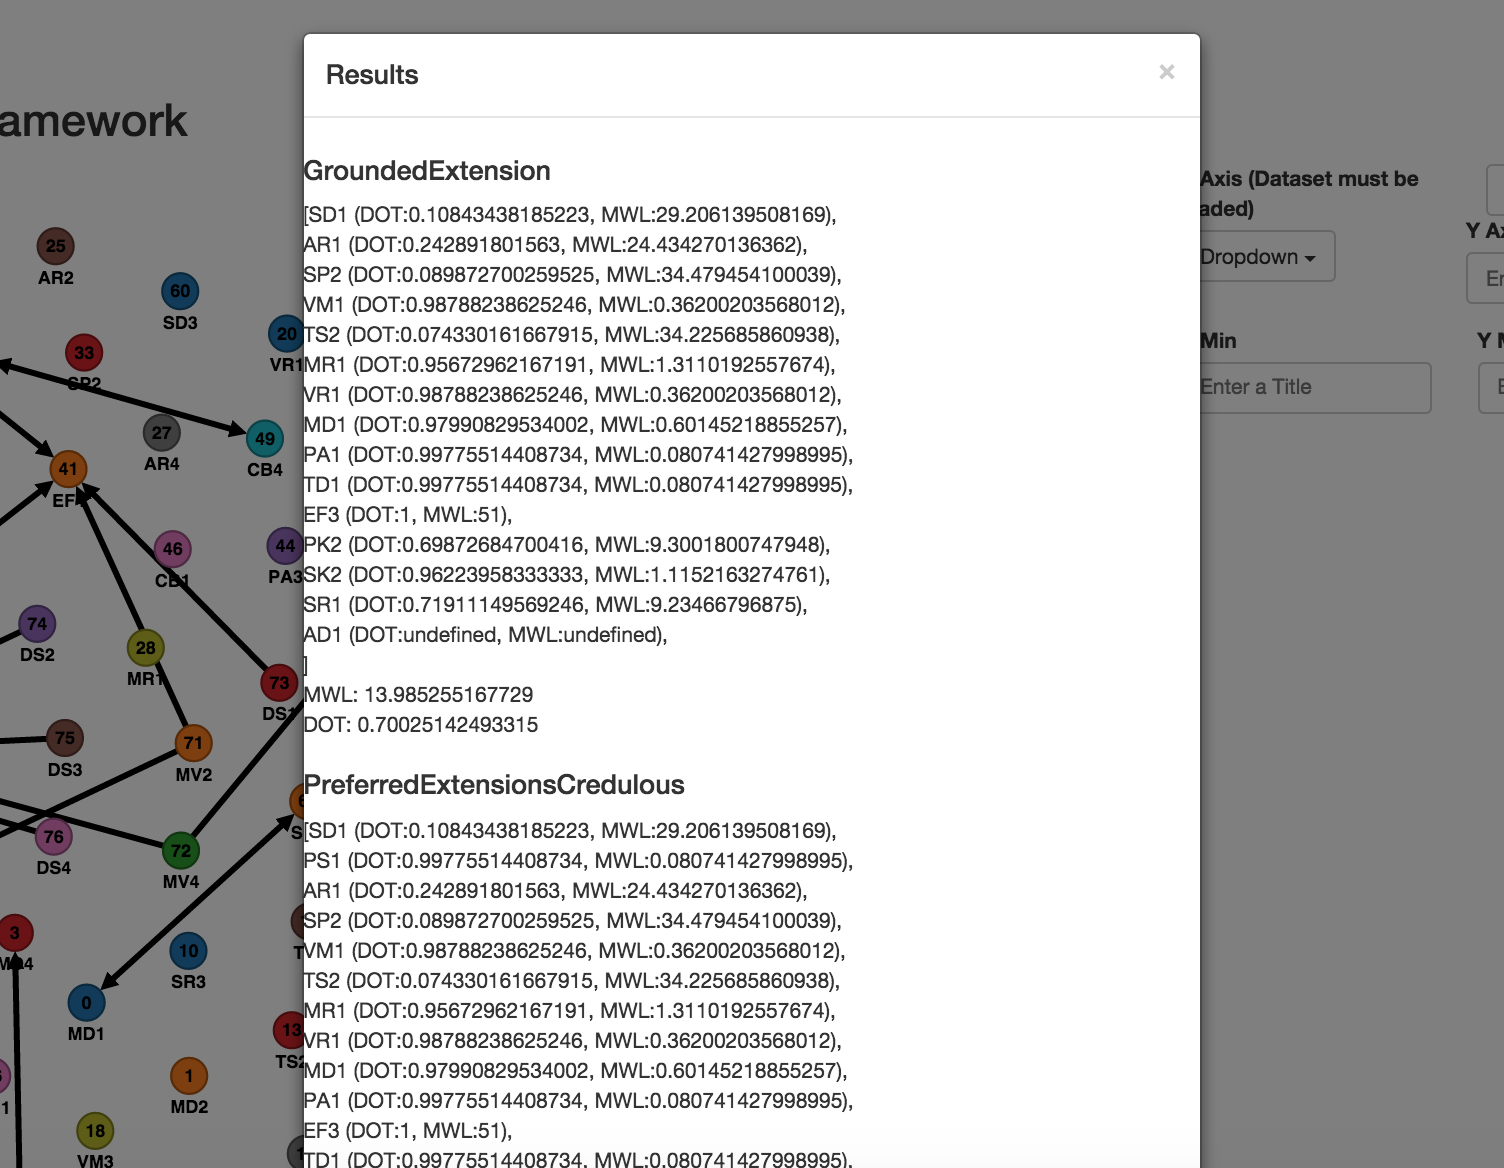
\includegraphics[width=1\textwidth]{results}
\caption{Results of computing the semantics on the framework}
\end{figure}

%----------------------------------------------------------------------------------------
%	SECTION 2
%----------------------------------------------------------------------------------------

\subsection{Generation of Results}



\section{Conclusions}



% Chapter Template

\chapter{Evaluation} % Main chapter title

\label{Chapter5} % Change X to a consecutive number; for referencing this chapter elsewhere, use \ref{ChapterX}

\lhead{Chapter 5. \emph{Evaluation}} % Change X to a consecutive number; this is for the header on each page - perhaps a shortened title



%----------------------------------------------------------------------------------------
%	RESULTS
%----------------------------------------------------------------------------------------

\section{Results}



%-----------------------------------
%	SUBSECTION 1
%-----------------------------------
\subsection{Predictive Capacity}


% These results are wrong. Fix them.
% dat = read.csv("texperimentnewer.csv", header = TRUE)
% threshold <- 0
% subset(dat, dat["time"] < threshold)
% colnames(dat[5:37])
% cor(dat[4:37])

\begin{center}
    \begin{tabular}{ | l | l | }
    \hline
    Technique & Correlation with time\\ \hline
    Amateur Knowledge Base Grounded Extension & 0.124536\\ \hline
    Amateur Knowledge Base Preferred Extension & 0.124536\\ \hline
    Expert Knowledge Base Grounded Extension & 0.2928288\\ \hline
    Expert Knowledge Base Preferred Extension & 0.2882237\\ \hline
    \end{tabular}
\end{center}


Time to compute simple knowledge base on 440 rows of data: 1m4.041s
Time to compute expert knowledge base on 440 rows of data: 1m44.001s


Why is the implementation slow?

PHP needs to spin up a new process for each row using exec and read the output.
Computing semantics is an NP complete problem.

%-----------------------------------
%	SUBSECTION 2
%-----------------------------------

\subsection{Classification}


%THIS IS STUPID, DON'T DO STUPID THINGS:
\begin{center}
    \begin{tabular}{ | l | l | l |}
    \hline
    Technique & Correlation with task ID \\ \hline
    Amateur Knowledge Base Grounded Extension & 0.09921536\\ \hline
    Amateur Knowledge Base Preferred Extension & 0.09921536\\ \hline
    Expert Knowledge Base Grounded Extension & 0.2056966\\ \hline
    Expert Knowledge Base Preferred Extension & 0.1986422\\ \hline
    \end{tabular}
\end{center}

\subsection{Minimum Description Length}



%----------------------------------------------------------------------------------------
%	SECTION 1
%----------------------------------------------------------------------------------------

\section{Evaluation}


%%% LIMITATIONS OF APPROACH - BEZIER CURVES CANT MODEL EXPONENTIAL PHENOMENA ETC... THIS COULD BE SUBJECT FOR FURTHER INVESTIGATION


%%% KNOWLEDGE ACQUISITION BOTTLENECK

%-----------------------------------
%	SUBSECTION 1
%-----------------------------------
\subsection{Subsection 1}

%-----------------------------------
%	SUBSECTION 2
%-----------------------------------

\subsection{Subsection 2}

Does this system encourage the development of a model that is too complex? Describe the knowledge base... An approach that emphasises simpler knowledge bases with fewer nodes is better.
%----------------------------------------------------------------------------------------
%	SECTION 2
%----------------------------------------------------------------------------------------

\section{Conclusions}


% Chapter Template

\chapter{Conclusions and Future Work} % Main chapter title

\label{Chapter6} 

\lhead{Chapter 6. \emph{Conclusions and Future Work}} 

This chapter revisits the aims of the projects. The key results of the research are summarised and their significance to answering the research question is discussed. The contribution of the research is made clear. Finally, areas for future research are outlined.

\section{Problem Definition and Research Overview}


\section{Experimentation, Evaluation and Limitations}

The central motive of this project is to compare and contrast machine learning with an implementation of defeasible reasoning. Specifically, the project examined the ability of the two techniques to measure a construct; in this case mental workload. Constructs by their nature are abstract and difficult to measure, so evaluating the performance of the techniques empirically is also a challenge. In order to determine that the techniques performed well two measures were taken which are widely used to assess the accuracy of measures; concurrent validity and convergent validity. Neither of these measures can conclusively tell us that the results are correct; they can only suggest to us that we are on the right path.

Although there was a limited amount of data to train and evaluate the techniques with, the results from the experiment can still provide us with some insight into the question posed at the start of the project. A core finding of this thesis is that supervised machine learning techniques are limited to learning to make predictions based on labeled training data. The only way to predict construct measures is to choose a field in the data and decide that this accurately measures the construct we are interested in. In the experiment, it was decided that MWL could be modeled using an objective performance measure, time. This approach was flawed, as it was shown that time had a poor convergent validity as a measure for MWL. From a practical point of view, this would suggest that if machine learning is to be used in an application to predict a construct, the data should be labeled or a column with a high convergent validity with other measures of the construct should be used. 

The convergent validity of the experts knowledge base was very high with respect to an existing measure of MWL. The non-expert's knowledge base had a high convergent validity with the existing measure of MWL as well, however, it was not nearly as strong as the expert's. This suggests that the implementation was providing a good representation of the construct and demonstrates the strength of defeasible reasoning for use in this situation.

The concurrent validity of the approaches was measured by their ability to predict an objective performance measure, time, and another objective value, task membership. It was believed that MWL would vary consistently across tasks as some tasks were designed to be more difficult than others. Predictions of task time made based on the MWL values computed from the expert's knowledge base were better than those of the amature and all but one machine learning approach. Over all, linear regression performed best at predicting task time. Predictions of task membership based on values for MWL from the knowledge based approach were found to be inaccurate. In this case logistic regression and naive bayes performed best. It is possible that task membership has a weak relationships with MWL. Unfortunately, as the task IDs are discrete values it is not possible to determine their convergent validity with other MWL measures. 

The performance of machine learning was likely hindered significantly by the limited amount of data available for training. It would be interesting to perform the experiments again with a larger data set. This highlights another strength of the defeasible reasoning approach, no training based on data is required. It is noted that the ability to verify a knowledge base against a data set is useful in the implementation of such a system as in this project. This requires a significantly smaller data set than that required to train a machine learning model. One criticism of knowledge based approaches is that they allow predictions to be made based on anecdotal evidence and not hard data. This is alleviated somewhat by the verification step in our approach. 

It was noted that this implementation of defeasible reasoning was particularly slow; implementation reasons for this have been identified. This approach may not be ready for real world implementation today, however, a hybrid approach using AT for data set labeling could be adopted as outlined in Appendix B. One of the main culprits of performance issues was the Dung-o-matic inference engine. It has been noted that other faster implementations exist but were not ready or available for integration in this project. This highlights a greater need within this argumentation theory community for an open source implementation of a library for computing argument semantics. This sentiment is shared by other authors who's work has been highlighted in the literature review.

The implementation of defeasible reasoning used in this project is (to my knowledge) the first implementation to adopt a graphical diagramming approach that is also used for computation of results. This has several possible advantages that could be investigated as the subject of future research. An expert could be trained in using the tool to elicit their knowledge base graphically which is likely more intuitive than inputting their knowledge base using some domain specific language. It is possible that in a similar fashion to the findings of \cite{twardy2004argument}, experts could improve their critical reasoning around their domain through interaction with the tool. It is also likely that through visualisation the comparison of knowledge bases will be made easier. 

\section{Contributions to the body of knowledge}

This project has highlighted a shortcoming of machine learning, the measurement of constructs, that can be better accomplished using a DR based approach. A key strength of argumentation theory over machine learning has been highlighted; that AT can allow experts to develop and evaluate constructs in an intuitive way.

The project provides a generalisable implementation of defeasible reasoning that is user friendly. It is the first implementation (to my knowledge) that integrates an argument diagramming approach with the computation of results. This implementation and its design can provide guidance to engineers and academics that seek to integrate these approaches into applications or their research.

\section{Future Work and Research}

In order to provide greater insight into the problem at hand the experiment could be carried out again with larger data sets across using different constructs. Further steps should be taken to optimised the DR implementation, including possible research into the efficient computation of argument semantics.

This project focused exclusively on supervised machine learning. An exploration of construct representation with unsupervised machine learning might provide new insights that have been ignored in this research.

The application developed in this project could itself be the subject of further research. The usability of the interface could be examined and whether it provides advantages in the elicitation of knowledge bases. In a similar manner to the work conducted by \cite{twardy2004argument} it could be interesting to examine whether or not an expert's understanding of their domain was improved through the knowledge elicitation process.


%----------------------------------------------------------------------------------------
%	THESIS CONTENT - APPENDICES
%----------------------------------------------------------------------------------------

\addtocontents{toc}{\vspace{2em}} % Add a gap in the Contents, for aesthetics

\appendix % Cue to tell LaTeX that the following 'chapters' are Appendices

% Include the appendices of the thesis as separate files from the Appendices folder
% Uncomment the lines as you write the Appendices

\setstretch{1.3} % Return the line spacing back to 1.3

% Appendix A

\chapter{Appendix Title Here} % Main appendix title

\label{AppendixA} % For referencing this appendix elsewhere, use \ref{AppendixA}

\lhead{Appendix A. \emph{Appendix Title Here}} % This is for the header on each page - perhaps a shortened title

Write your Appendix content here.
%% Appendix Template

\chapter{Appendix Title Here} % Main appendix title

\label{AppendixB} % Change X to a consecutive letter; for referencing this appendix elsewhere, use \ref{AppendixX}

\lhead{Appendix B. \emph{Note on Time to Compute}} 

It should be noted that the implementation of the DR system has a significantly higher time to compute than the machine learning techniques as shown in table ~\ref{tab:timeperformance}.

\begin{table}[!htbp]
\centering
\begin{tabular}{|c|c|}
\hline
 & Time to compute results \\ \hline
Regression Techniques & \\ \hline
Simple Linear Regression & 0m0.001s\\
Decision Table & 0m0.71s\\
K Star & 0m0.001s\\
Additive Regression & 0m0.05s\\
Linear Regression & 0m0.01s\\ \hline
Classification Techniques & \\ \hline
Bayes Net &0m0.02s \\
Decision Table & 0m0.08s\\  
Logistic Regression & 0m01.37s\\ 
Naive Bayes & 0m0.02s\\ 
Random Tree & 0m0.03s\\ \hline
Defeasible Reasoning & \\ \hline
Peter KB & 1m4.041s\\
Luca KB & 1m44.001s\\
\hline
\end{tabular}
\caption{Time to compute results of techniques}
\label{tab:timeperformance}
\end{table}

There are a number of contributing factors that explain the poor performance of the defeasible reasoning system that could be resolved in future implementations. 

There are a number of performance issues specific to this implementation. In order to compute the semantics of an AF the PHP code uses exec to start a new Java process. Creating a new process for each iteration is resource consuming and has a costly overhead associated with it. This could be solved in future implementation by developing the whole server application in Java or by creating a separate long running Java service that can compute the semantics on demand. The implementation trades some performance for speed of development by using PHP as a server side language. The process of determining output values for membership and output functions also adds an overhead to the computation. This has been reduced somewhat by caching previously computed values for nodes. 

The other culprit that is diminishing performance in the implementation is the Dung-o-matic. It has been highlighted by \cite{cerutti2014generating} that the Dung-o-matic implementation doesn't perform as well as other implementations. It is unfortunate that the other implementations are unavailable and it would be interesting to evaluate the performance of the system using a different argumentation engine. It is important to keep in mind that the computation of these semantics is an NP complete problem. The time to compute the results grows massively with the number of nodes in the knowledge base. It would be interesting to evaluate the performance and accuracy of the approach if the expert was instructed to restrain the size of their knowledge base by merging some arguments.

While the above results demonstrate a trade off between machine learning techniques and defeasible reasoning ones, the defeasible reasoning system isn't obsolete as a result of the performance overhead. This will be clarified in the next chapter.
%\input{Appendices/AppendixC}

\addtocontents{toc}{\vspace{2em}} % Add a gap in the Contents, for aesthetics

\backmatter

%----------------------------------------------------------------------------------------
%	BIBLIOGRAPHY
%----------------------------------------------------------------------------------------

\label{Bibliography}

\lhead{\emph{Bibliography}} % Change the page header to say "Bibliography"

\bibliographystyle{unsrtnat} % Use the "unsrtnat" BibTeX style for formatting the Bibliography

\bibliography{Bibliography} % The references (bibliography) information are stored in the file named "Bibliography.bib"

\end{document}
